\documentclass[a4paper, 11pt]{article}
\usepackage{fullpage} % changes the margin
 
\usepackage[english]{babel}
\usepackage[utf8]{inputenc}
\usepackage{graphicx}
\graphicspath{{./}{./plots/}{./plots/task2a/}{./plots/task2b/}}
\usepackage{booktabs}
\usepackage{float}
\usepackage{caption}
\usepackage{subcaption}
\usepackage{xcolor}
 
\usepackage{verbatim}

\usepackage{amsmath}
\usepackage{amsfonts}
\usepackage{amssymb}
\usepackage{hyperref}

\hypersetup{
    colorlinks=true,
    linkcolor=blue,
    urlcolor=cyan
}
 
\begin{document}
\noindent
\large\textbf{Report: Assignment 2} \hfill \textit{Team Name: }\textbf{Cache Us} \\
\normalsize CS683 - Advanced Computer Architecture \hfill IIT Bombay \\
Prof. Biswabandan Panda \hfill \today \\
Dept. Computer Science \& Engineering \hfill Indian Institute of Technology Bombay
 
\vspace{0.5em}
\hrule
\vspace{0.8em}
 
\tableofcontents
\vspace{1em}
\hrule
\vspace{1.5em}
 
\section{Data Prefetching}
\subsection{Understanding IP stride code}
The IP-stride prefetcher tracks memory accesses separately for each instruction pointer (IP). It stores the previous cache block address, observed stride, and LRU information.

For each access, it calculates the stride between the current and previous block addresses. If consecutive strides match, it predicts future addresses and issues prefetch requests for up to three blocks.

The prefetcher avoids crossing 4 KB page boundaries and selects L1 or L2 as the prefetch destination based on MSHR occupancy. When the tracking table is full, it replaces the least-recently-used entry.

Thus, it exploits regular memory access patterns to fetch data in advance, while irregular or changing strides can reduce its effectiveness.
\subsection{Stride Pattern Prefetching (SPP)}
\begin{itemize}
    \item \textbf{IPC, Speedup, L1D Load MPKI, Prefetch Accuracy, and Coverage Values:}
    
    \begin{table}[H]
\centering
\caption{Performance evaluation of the Stride Pattern Prefetcher (SPP) compared against Baseline.}
\label{tab:spp-results}
\resizebox{\textwidth}{!}{
\begin{tabular}{lccccccc}
\toprule
Trace & Baseline IPC & SPP IPC & Speedup & Baseline L1D MPKI & SPP L1D MPKI & Prefetch Accuracy & Coverage \\
\midrule
Trace 1 & 0.2321 & 0.2338 & 1.0073$\times$ (+0.73\%) & 10.6788 & 9.6901 & 53.48\% & 9.26\% \\
Trace 2 & 0.2500 & 0.2511 & 1.0046$\times$ (+0.46\%) & 13.5372 & 13.2056 & 46.03\% & 2.45\% \\
Trace 3 & 0.3819 & 0.3883 & 1.0168$\times$ (+1.68\%) & 3.4036 & 2.9145 & 44.96\% & 14.37\% \\
\bottomrule
\end{tabular}
}
\end{table}

For comparison, the reference IP-stride prefetcher achieves an IPC of 0.2331 (1.0043$\times$), 0.2501 (1.0006$\times$), and 0.3827 (1.0021$\times$) on Traces 1, 2, and 3, respectively. SPP consistently outperforms IP-stride across all benchmarks in both speedup and coverage due to its dual pattern classification and multi-stride lookahead capability.

\begin{figure}[H]
    \centering
    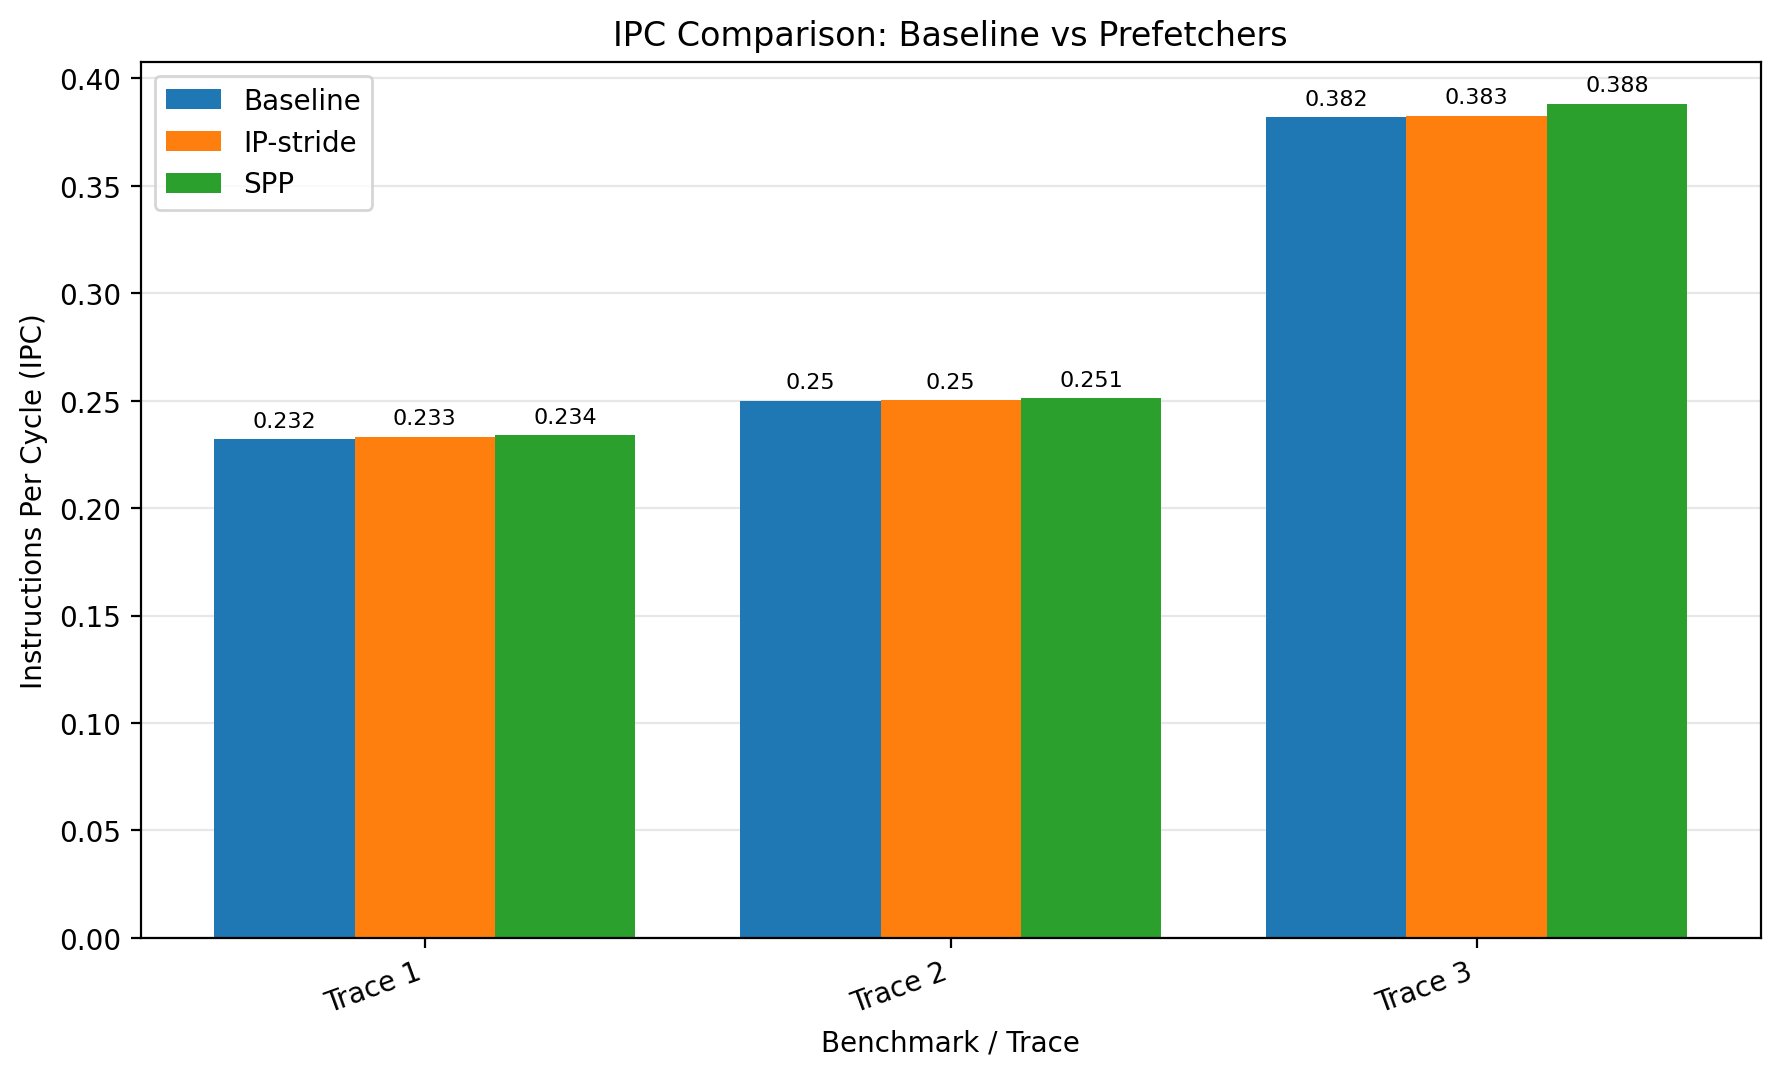
\includegraphics[width=0.85\textwidth]{ipc_plot.png}
    \caption{IPC comparison across Baseline, IP-stride, and SPP.}
    \label{fig:spp-ipc}
\end{figure}

\begin{figure}[H]
    \centering
    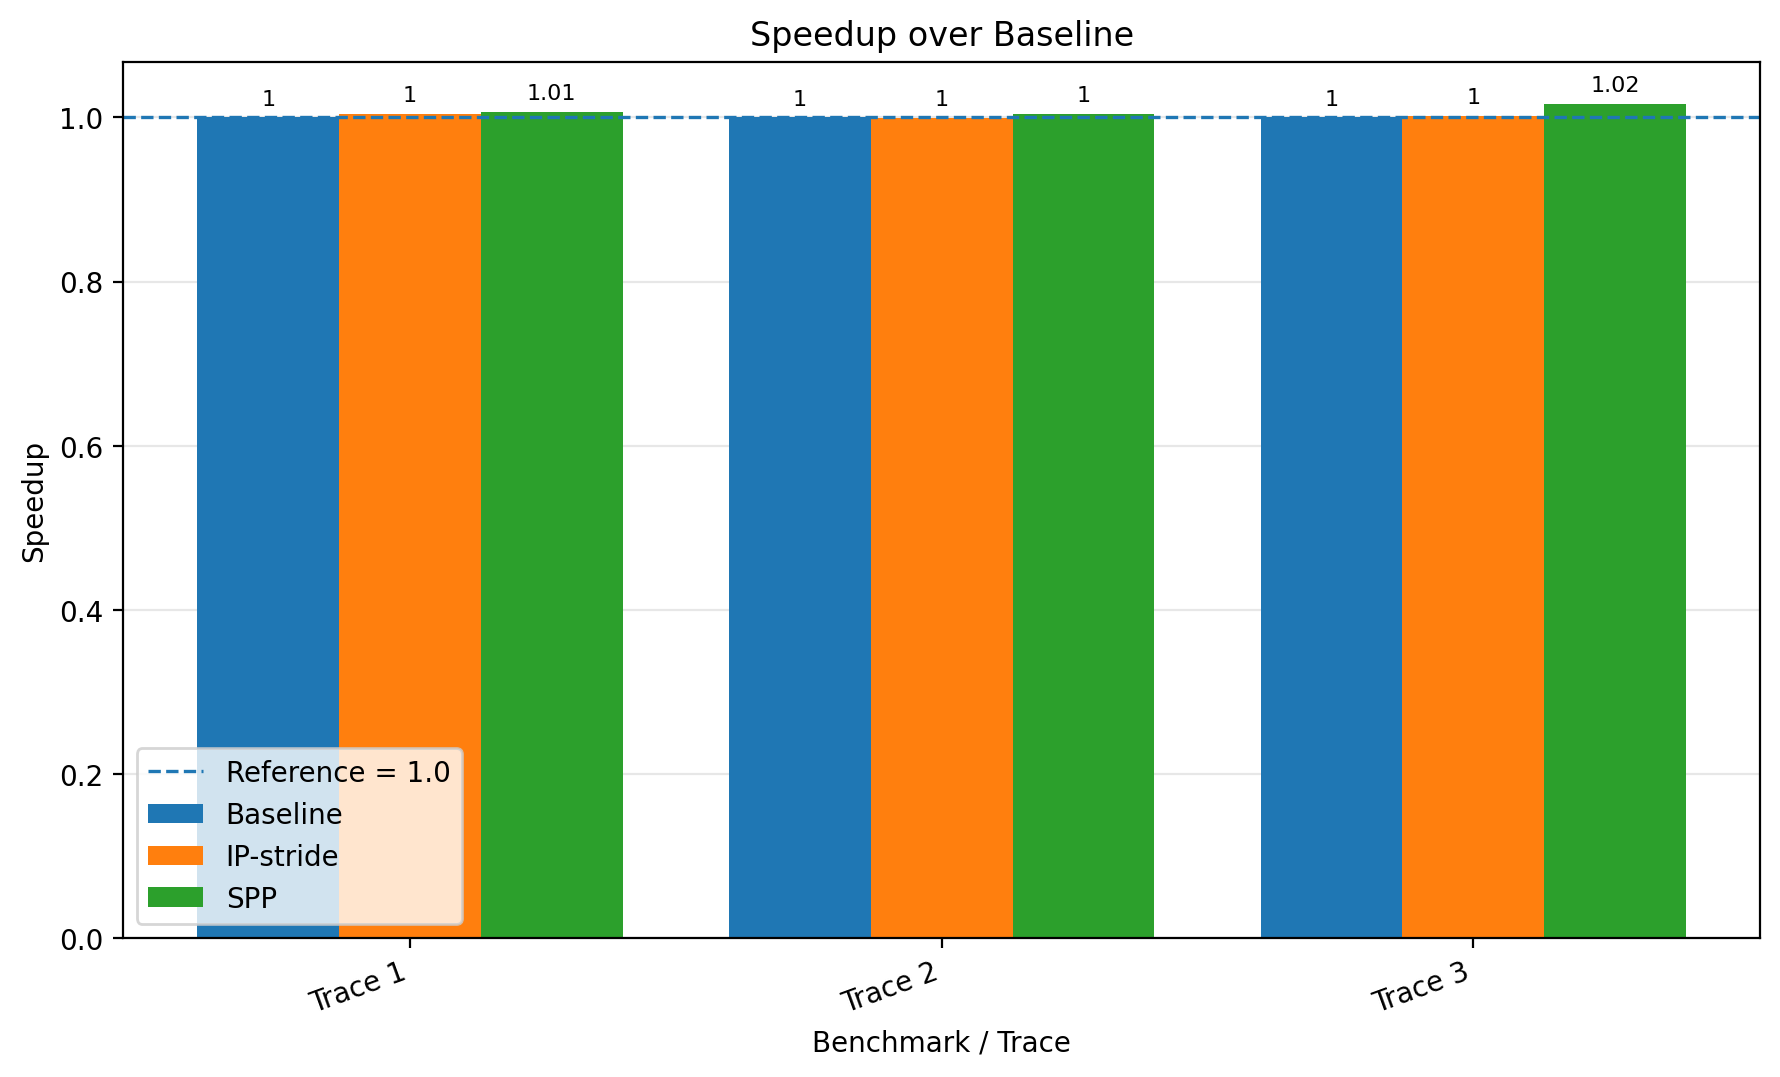
\includegraphics[width=0.85\textwidth]{speedup_plot.png}
    \caption{Speedup comparison of SPP against the baseline and IP-stride.}
    \label{fig:spp-speedup}
\end{figure}

\begin{figure}[H]
    \centering
    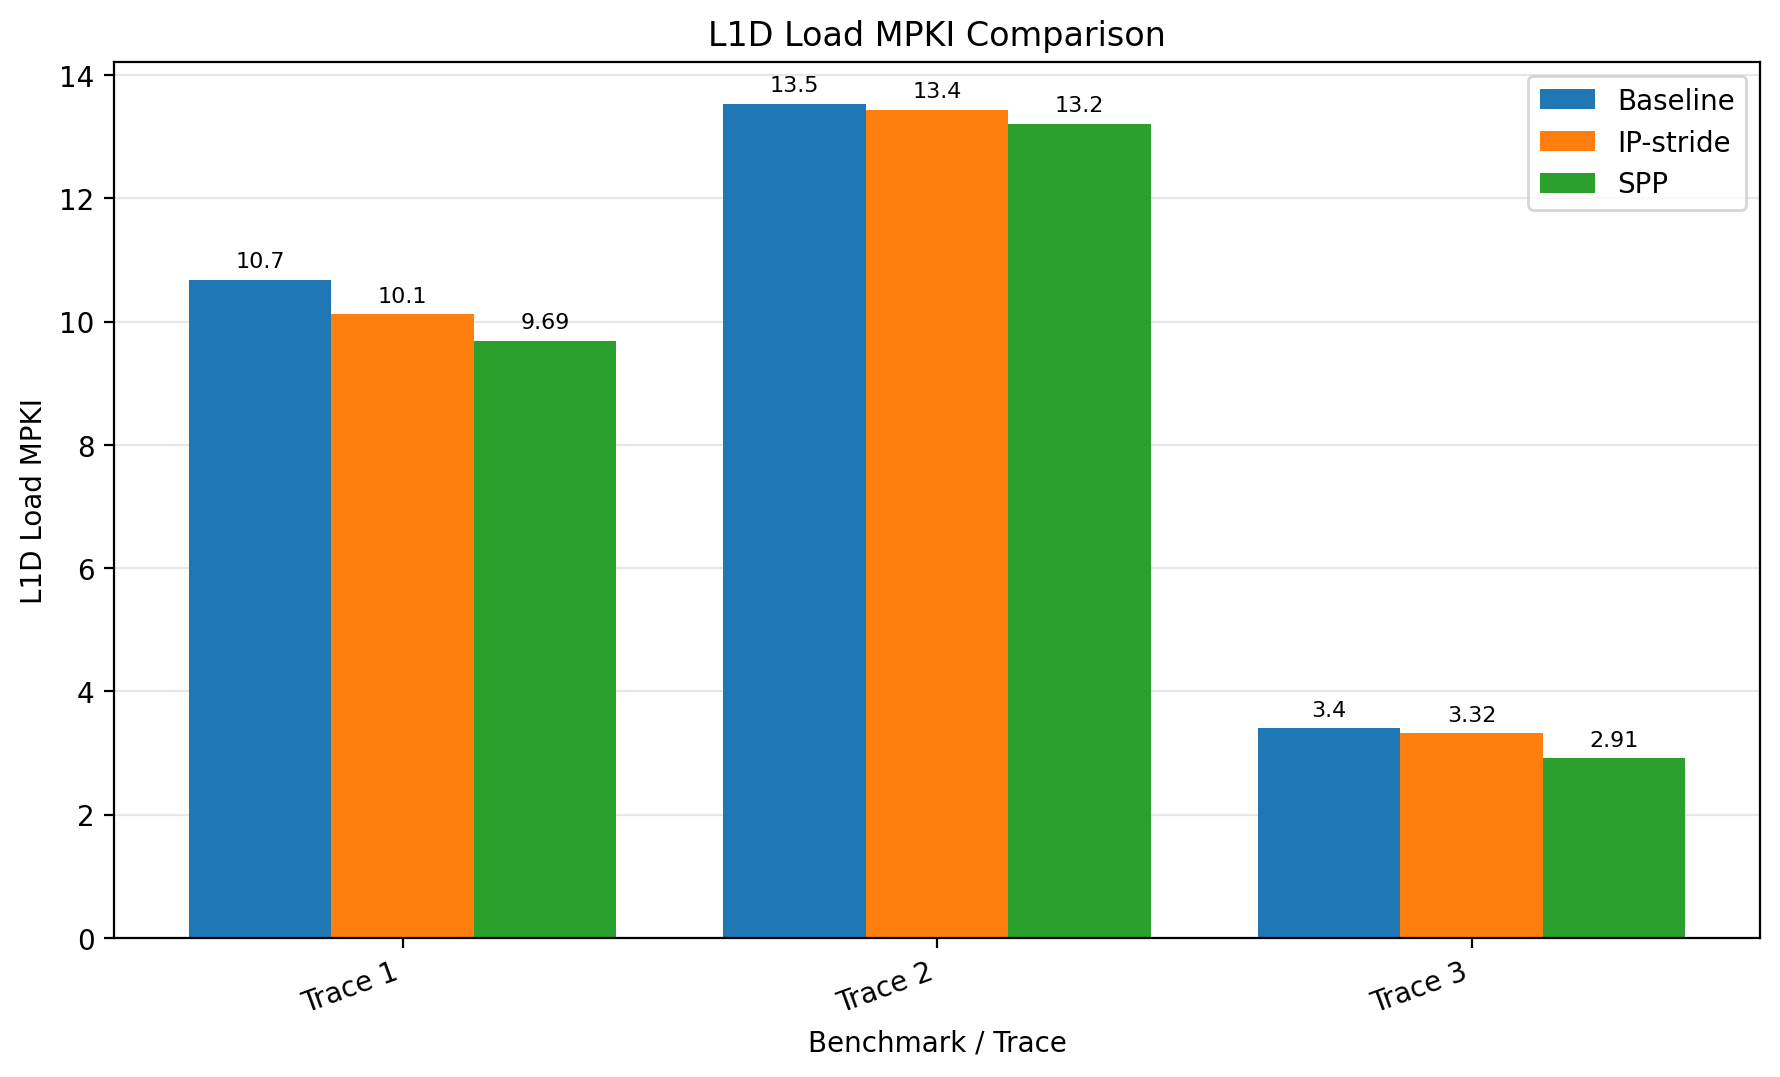
\includegraphics[width=0.85\textwidth]{mpki_plot.png}
    \caption{L1D Load MPKI comparison across Baseline, IP-stride, and SPP.}
    \label{fig:spp-mpki}
\end{figure}

\begin{figure}[H]
    \centering
    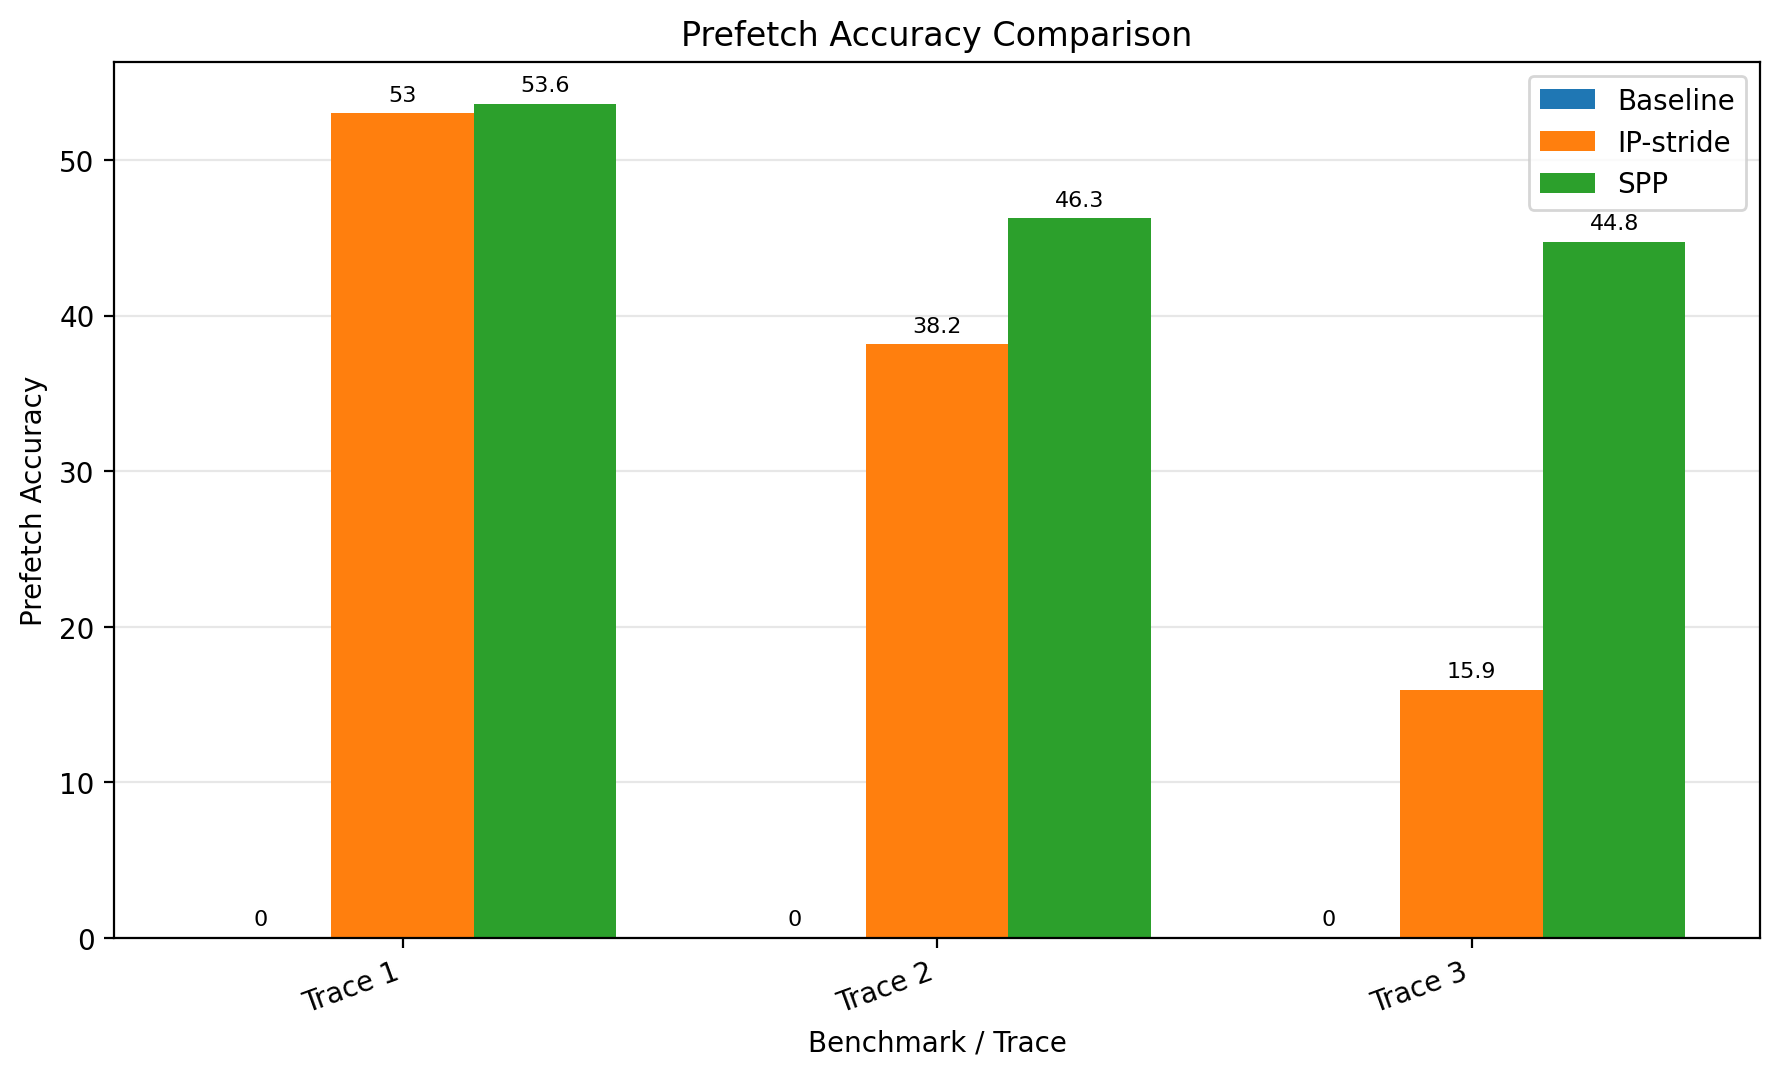
\includegraphics[width=0.85\textwidth]{accuracy_plot.png}
    \caption{Prefetch accuracy across benchmark traces.}
    \label{fig:spp-accuracy}
\end{figure}

\begin{figure}[H]
    \centering
    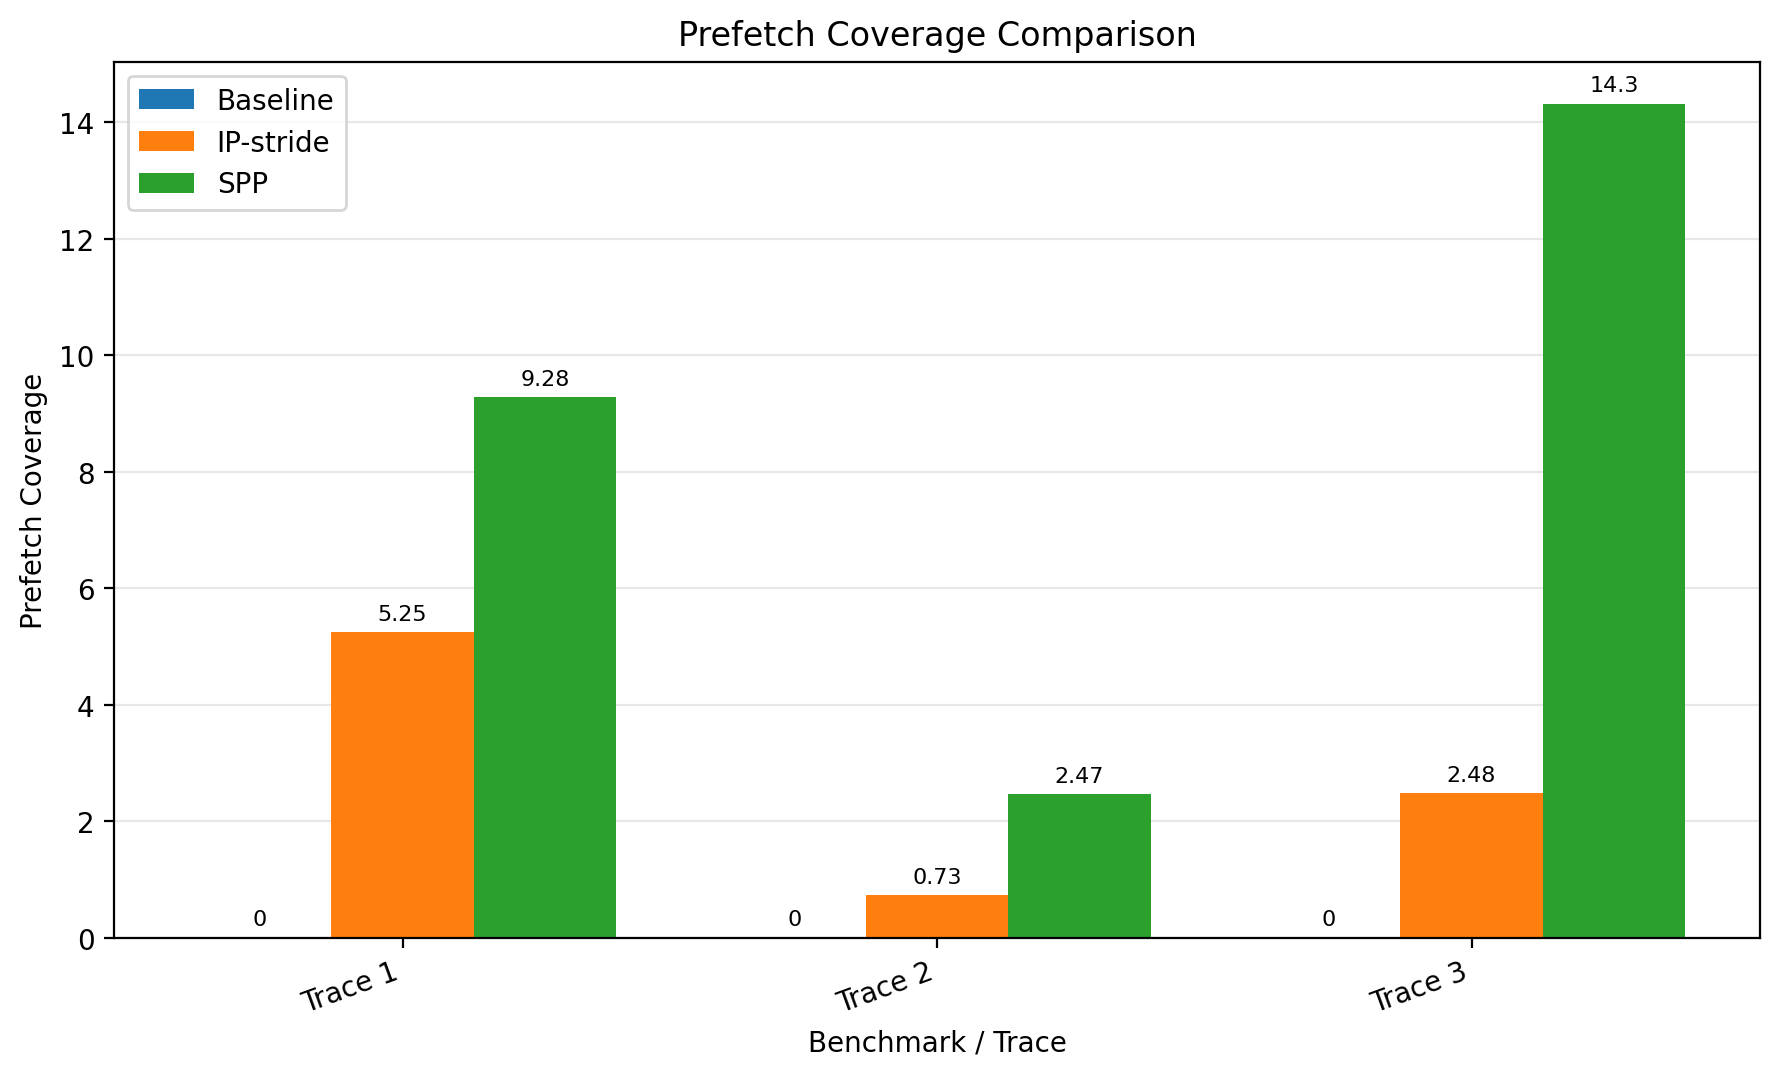
\includegraphics[width=0.85\textwidth]{coverage_plot.png}
    \caption{L1D prefetch coverage across benchmark traces.}
    \label{fig:spp-coverage}
\end{figure}

    \item \textbf{Total Storage Overhead of Prefetcher:}
    
    The prefetcher consists of two primary hardware tables and a minimal set of control registers:
    \begin{table}[H]
\centering
\caption{Bit-level storage overhead of the Stride Pattern Prefetcher (SPP).}
\label{tab:spp-storage}
\begin{tabular}{llccc}
\toprule
Table & Field & Bits per Entry & Number of Entries & Total Bits \\
\midrule
\textbf{IP Tracking Table} & Valid bit & 1 & 64 & 64 \\
                           & IP Tag (\texttt{ip \& 0xFFFF}) & 16 & 64 & 1,024 \\
                           & Last Cache Line Address & 58 & 64 & 3,712 \\
                           & Last Observed Stride & 8 & 64 & 512 \\
                           & Uniform Confidence Counter & 2 & 64 & 128 \\
                           & Stride History Signature & 10 & 64 & 640 \\
                           & LRU Replacement State & 6 & 64 & 384 \\
\midrule
\multicolumn{2}{l}{\textit{IP Table Subtotal}} & \textit{101 bits} & \textit{64} & \textit{6,464 bits (808 B)} \\
\midrule
\textbf{Pattern Table (PT)} & Predicted Next Stride & 8 & 1,024 & 8,192 \\
                            & Prediction Confidence Counter & 2 & 1,024 & 2,048 \\
\midrule
\multicolumn{2}{l}{\textit{Pattern Table Subtotal}} & \textit{10 bits} & \textit{1,024} & \textit{10,240 bits (1,280 B)} \\
\midrule
\textbf{Control Registers}  & Last Epoch Issued Counter & 32 & 1 & 32 \\
                            & Last Epoch Useful Counter & 32 & 1 & 32 \\
                            & Current Dynamic Degree Register & 3 & 1 & 3 \\
\midrule
\multicolumn{2}{l}{\textit{Control Registers Subtotal}} & \textit{67 bits} & \textit{1} & \textit{67 bits (~8.4 B)} \\
\midrule
\multicolumn{4}{r}{\textbf{Total Storage Overhead}} & \textbf{16,771 bits (2,096.4 B $\approx$ 2.05 KB)} \\
\bottomrule
\end{tabular}
\end{table}

    \item \textbf{Threshold for Accuracy Throttling:}
    \begin{itemize}
        \item \textbf{What:} Accuracy throttling evaluates the usefulness of issued prefetches dynamically over sliding evaluation epochs of $\text{ACC\_CHECK\_INTERVAL} = 256$ issued prefetches using hardware performance counters ($\Delta \text{pf\_useful}$ and $\Delta \text{pf\_issued}$):
        \begin{equation}
            \text{Accuracy} = \frac{\Delta \text{pf\_useful}}{\Delta \text{pf\_issued}} \times 100\%
        \end{equation}
        The prefetcher partitions operation into four accuracy regions using three static decision thresholds:
        \begin{itemize}
            \item \textbf{High Accuracy ($\ge 70\%$):} Prefetches are hitting with high probability.
            \item \textbf{Medium Accuracy ($45\% \le \text{Accuracy} < 70\%$):} Good prefetch usefulness with modest miss penalty.
            \item \textbf{Low Accuracy ($25\% \le \text{Accuracy} < 45\%$):} Marginal prefetch usefulness; higher risk of displacing active cache lines.
            \item \textbf{Critical / Poor Accuracy ($< 25\%$):} Fewer than 1 in 4 prefetches hit; prefetching is predominantly causing cache pollution and queue contention.
        \end{itemize}
        
        \item \textbf{Why:} An interval of 256 prefetches provides agile tracking of rapid application phase shifts while dampening transient noise. The chosen thresholds (70\%, 45\%, and 25\%) balance memory latency hiding against cache pollution:
        \begin{itemize}
            \item When accuracy exceeds 70\%, prefetching is highly effective and rarely evicts useful demand lines, justifying aggressive lookahead.
            \item In the 45\%--70\% range, moderate prefetching provides substantial coverage without congesting L1D MSHR entries.
            \item When accuracy falls below 25\%, more than 75\% of prefetched lines are evicting demand data before being used, necessitating strict throttling to prevent severe IPC degradation.
        \end{itemize}
    \end{itemize}

    \item \textbf{Prefetch Degrees for the Different Accuracy Ranges:}
    
    \begin{table}[H]
\centering
\caption{Prefetch degrees assigned to each dynamic accuracy range.}
\label{tab:spp-degree-throttling}
\begin{tabular}{lcl}
\toprule
Accuracy Range & Prefetch Degree & Operating Mode / Rationale \\
\midrule
$\ge 70\%$ & 4 & Aggressive prefetching; chains deep lookahead to hide long memory latency \\
$45\% \le \text{Accuracy} < 70\%$ & 3 & Balanced prefetching; matches standard IP-stride aggressiveness \\
$25\% \le \text{Accuracy} < 45\%$ & 2 & Conservative lookahead; curbs speculative depth to limit cache pollution \\
$< 25\%$ & 1 & Heavy throttling; issues only the immediate next block to prevent thrashing \\
\bottomrule
\end{tabular}
\end{table}

    \textbf{Rationale for Selected Degrees:}
    \begin{itemize}
        \item \textbf{Degree 4 ($\ge 70\%$):} When confidence and accuracy are high, chaining lookahead through 4 consecutive strides in the Pattern Table (e.g., $(+1, +2, +2, +2)$) pulls data far in advance, completely overlapping L1 miss latency (~10--15 CPU cycles to L2) without stalling the execution core.
        \item \textbf{Degree 3 ($45\% \le \text{Accuracy} < 70\%$):} Serves as the balanced operating baseline (matching the default degree of IP-stride). It maintains high bandwidth throughput while staying comfortably within the L1D prefetch queue capacity (PQ size of 16 entries).
        \item \textbf{Degree 2 ($25\% \le \text{Accuracy} < 45\%$):} Reduces speculative lookahead depth when stride transitions become irregular. Fetching only 2 blocks bounds cache line displacement while still prefetching ahead of the CPU demand stream by one extra cache line.
        \item \textbf{Degree 1 ($< 25\%$):} Acts as a protective lower bound. Rather than turning off prefetching entirely (which would prevent the Pattern Table from training and recovering when the program enters a new phase), Degree 1 only probes the immediate single stride, maintaining zero cache thrashing until accuracy improves.
    \end{itemize}

\end{itemize}


\section{Cache Replacement Policy}
\subsection{Instruction-Conscious L2 Replacement Policy (I-RRIP)}
\subsubsection{IPC, Speedup, and Load MPKI Results}

\begin{table}[H]
\centering
\caption{IPC and Speedup comparison across Baseline (LRU), RRIP, and I-RRIP.}
\label{tab:irrip-performance}
\resizebox{\textwidth}{!}{
\begin{tabular}{lcccccc}
\toprule
& \multicolumn{3}{c}{IPC} & \multicolumn{3}{c}{Speedup over Baseline} \\
\cmidrule(lr){2-4} \cmidrule(lr){5-7}
Trace & Baseline (LRU) & RRIP & I-RRIP & Baseline (LRU) & RRIP & I-RRIP \\
\midrule
Trace 1 & 0.2323 & 0.2323 & 0.2357 & 1.0000$\times$ & 1.0001$\times$ (+0.01\%) & 1.0148$\times$ (+1.48\%) \\
Trace 2 & 0.2506 & 0.2513 & 0.2603 & 1.0000$\times$ & 1.0026$\times$ (+0.26\%) & 1.0385$\times$ (+3.85\%) \\
Trace 3 & 0.3820 & 0.3816 & 0.3844 & 1.0000$\times$ & 0.9990$\times$ (-0.10\%) & 1.0062$\times$ (+0.62\%) \\
\bottomrule
\end{tabular}
}
\end{table}

\begin{table}[H]
\centering
\caption{L2 Load MPKI comparison across Baseline (LRU), RRIP, and I-RRIP.}
\label{tab:irrip-mpki}
\resizebox{\textwidth}{!}{
\begin{tabular}{lccccccccc}
\toprule
& \multicolumn{3}{c}{Baseline (LRU)} & \multicolumn{3}{c}{RRIP} & \multicolumn{3}{c}{I-RRIP} \\
\cmidrule(lr){2-4} \cmidrule(lr){5-7} \cmidrule(lr){8-10}
Trace & L2C MPKI & L2I MPKI & L2D MPKI & L2C MPKI & L2I MPKI & L2D MPKI & L2C MPKI & L2I MPKI & L2D MPKI \\
\midrule
Trace 1 & 17.7509 & 10.4030 & 7.3479 & 17.6814 & 10.6129 & 7.0684 & 19.0249 & 9.0044 & 10.0204 \\
Trace 2 & 28.2286 & 19.5298 & 8.6988 & 26.6066 & 18.5456 & 8.0610 & 21.6864 & 9.2780 & 12.4084 \\
Trace 3 & 3.9592 & 1.1232 & 2.8360 & 4.0443 & 1.1976 & 2.8467 & 3.9884 & 0.7153 & 3.2731 \\
\bottomrule
\end{tabular}
}
\end{table}

\begin{figure}[H]
    \centering
    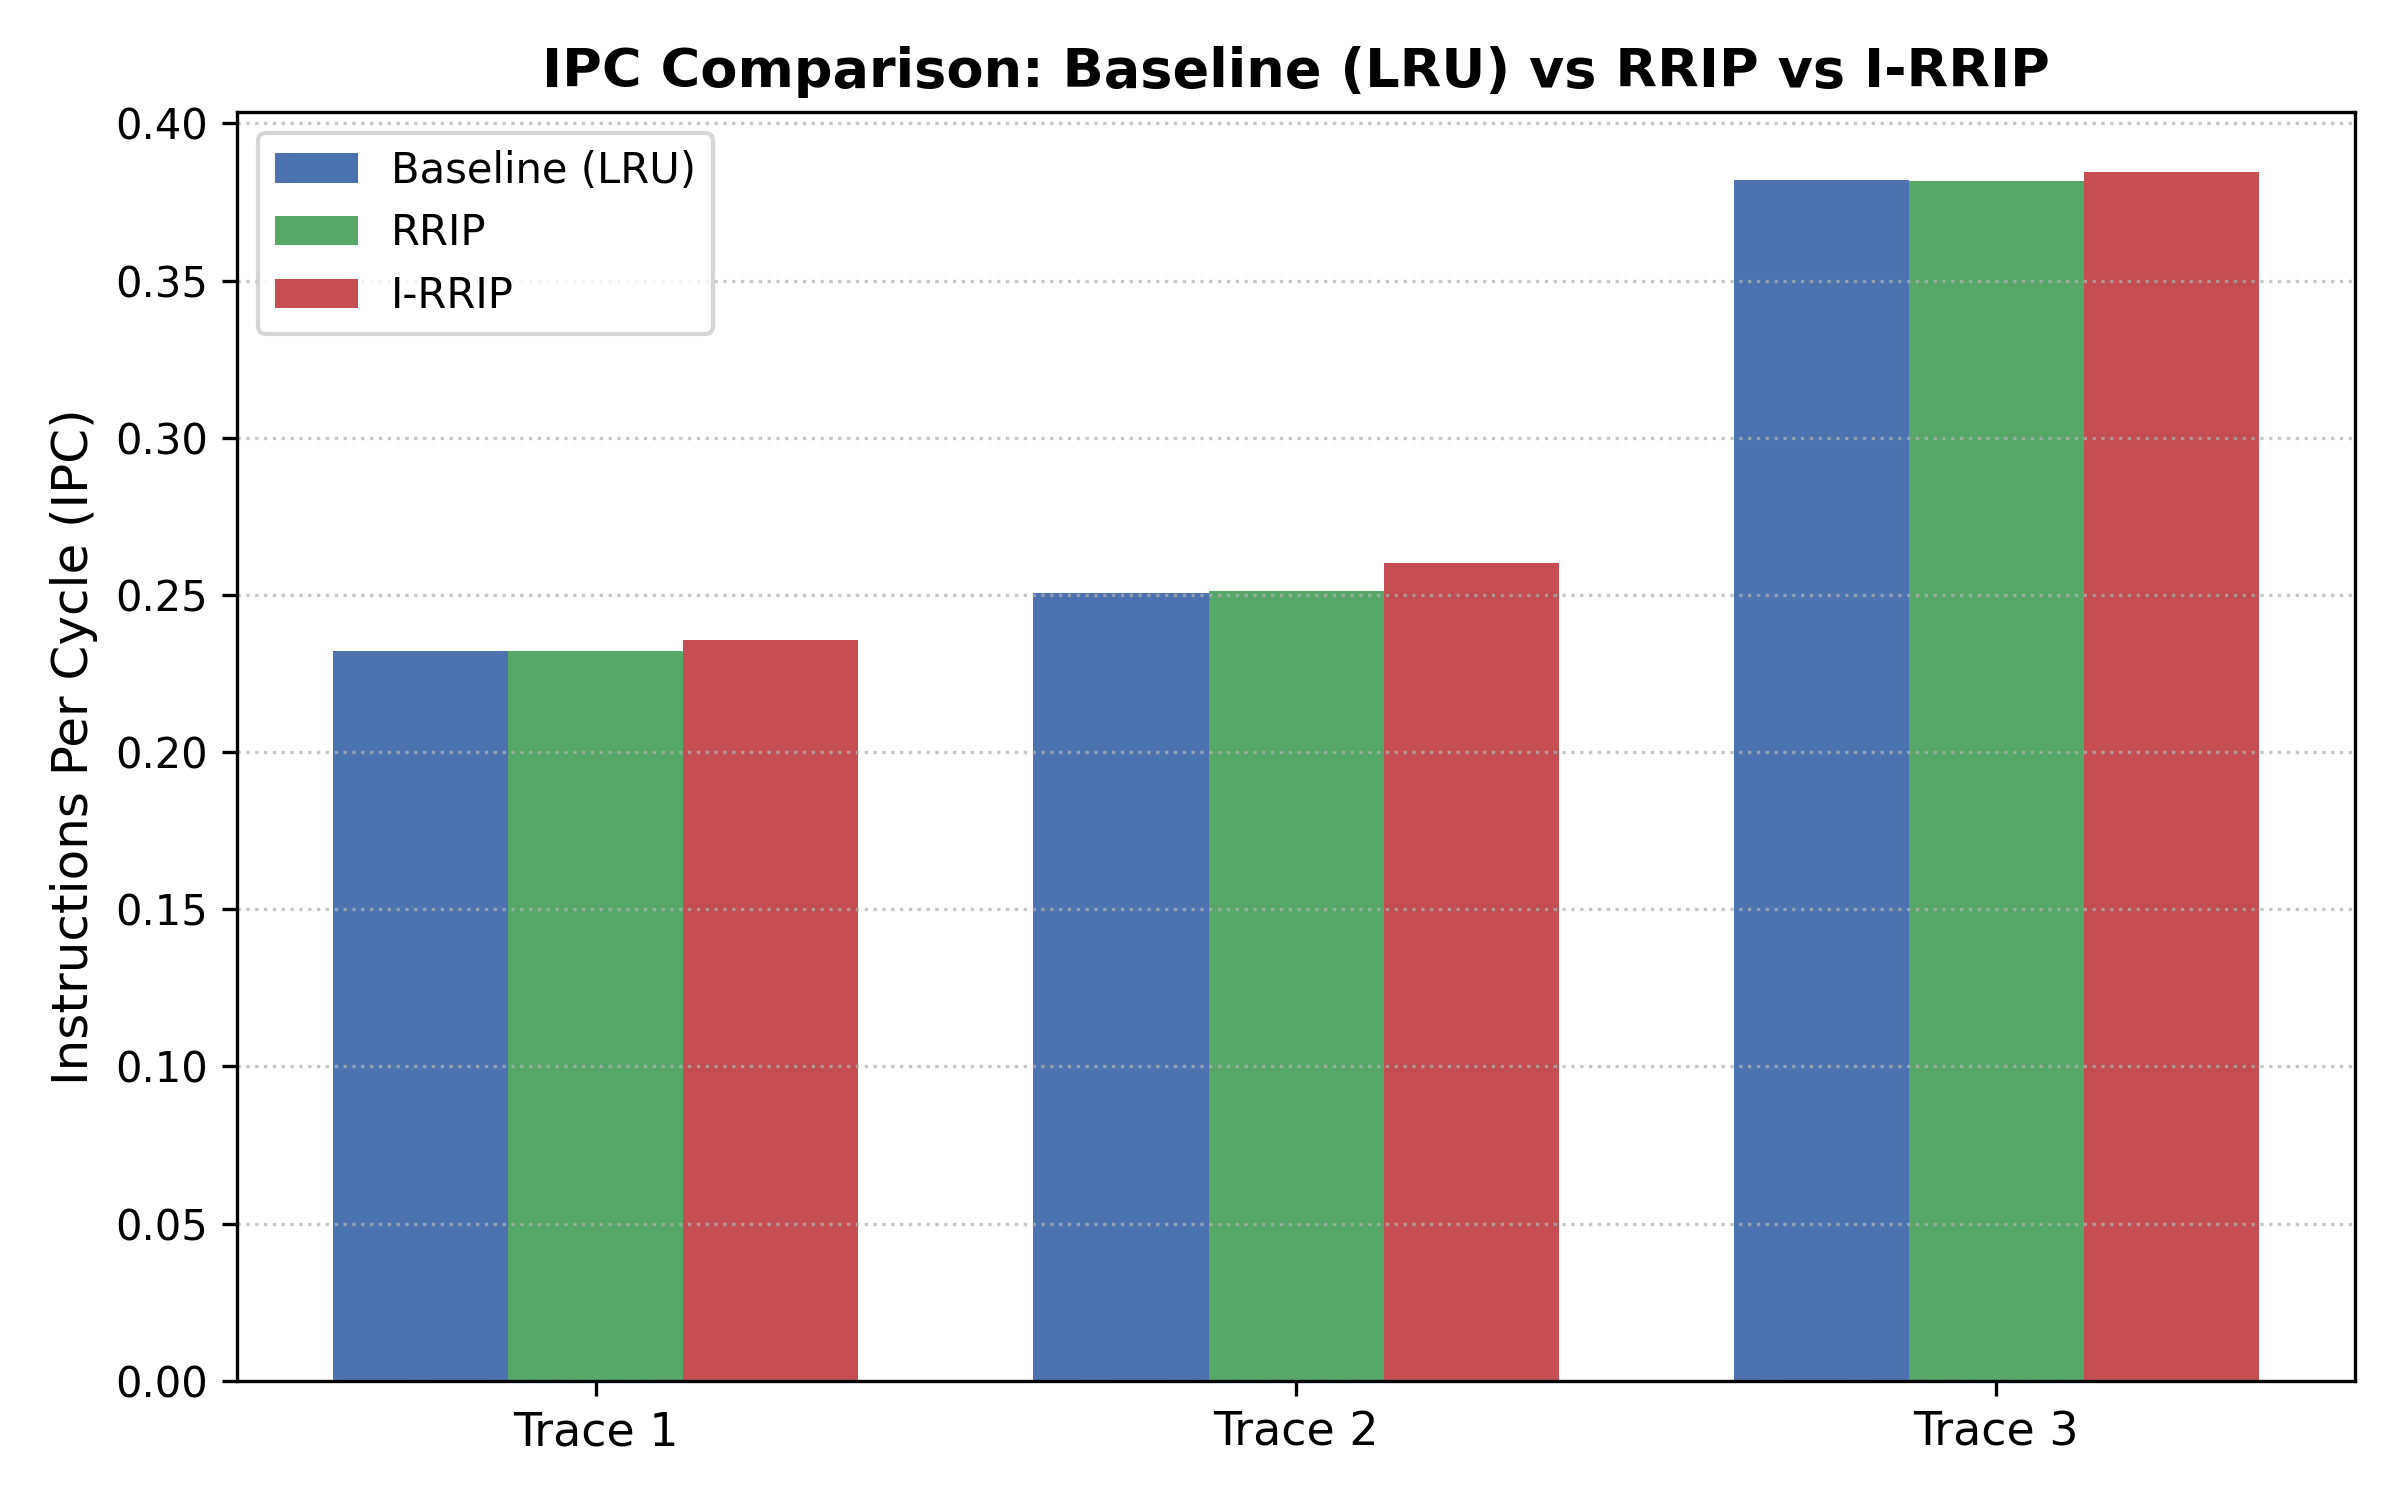
\includegraphics[width=0.85\textwidth]{plots/task2a/task2a_ipc.png}
    \caption{IPC comparison across Baseline (LRU), RRIP, and I-RRIP across benchmark traces.}
    \label{fig:task2a-ipc}
\end{figure}

\begin{figure}[H]
    \centering
    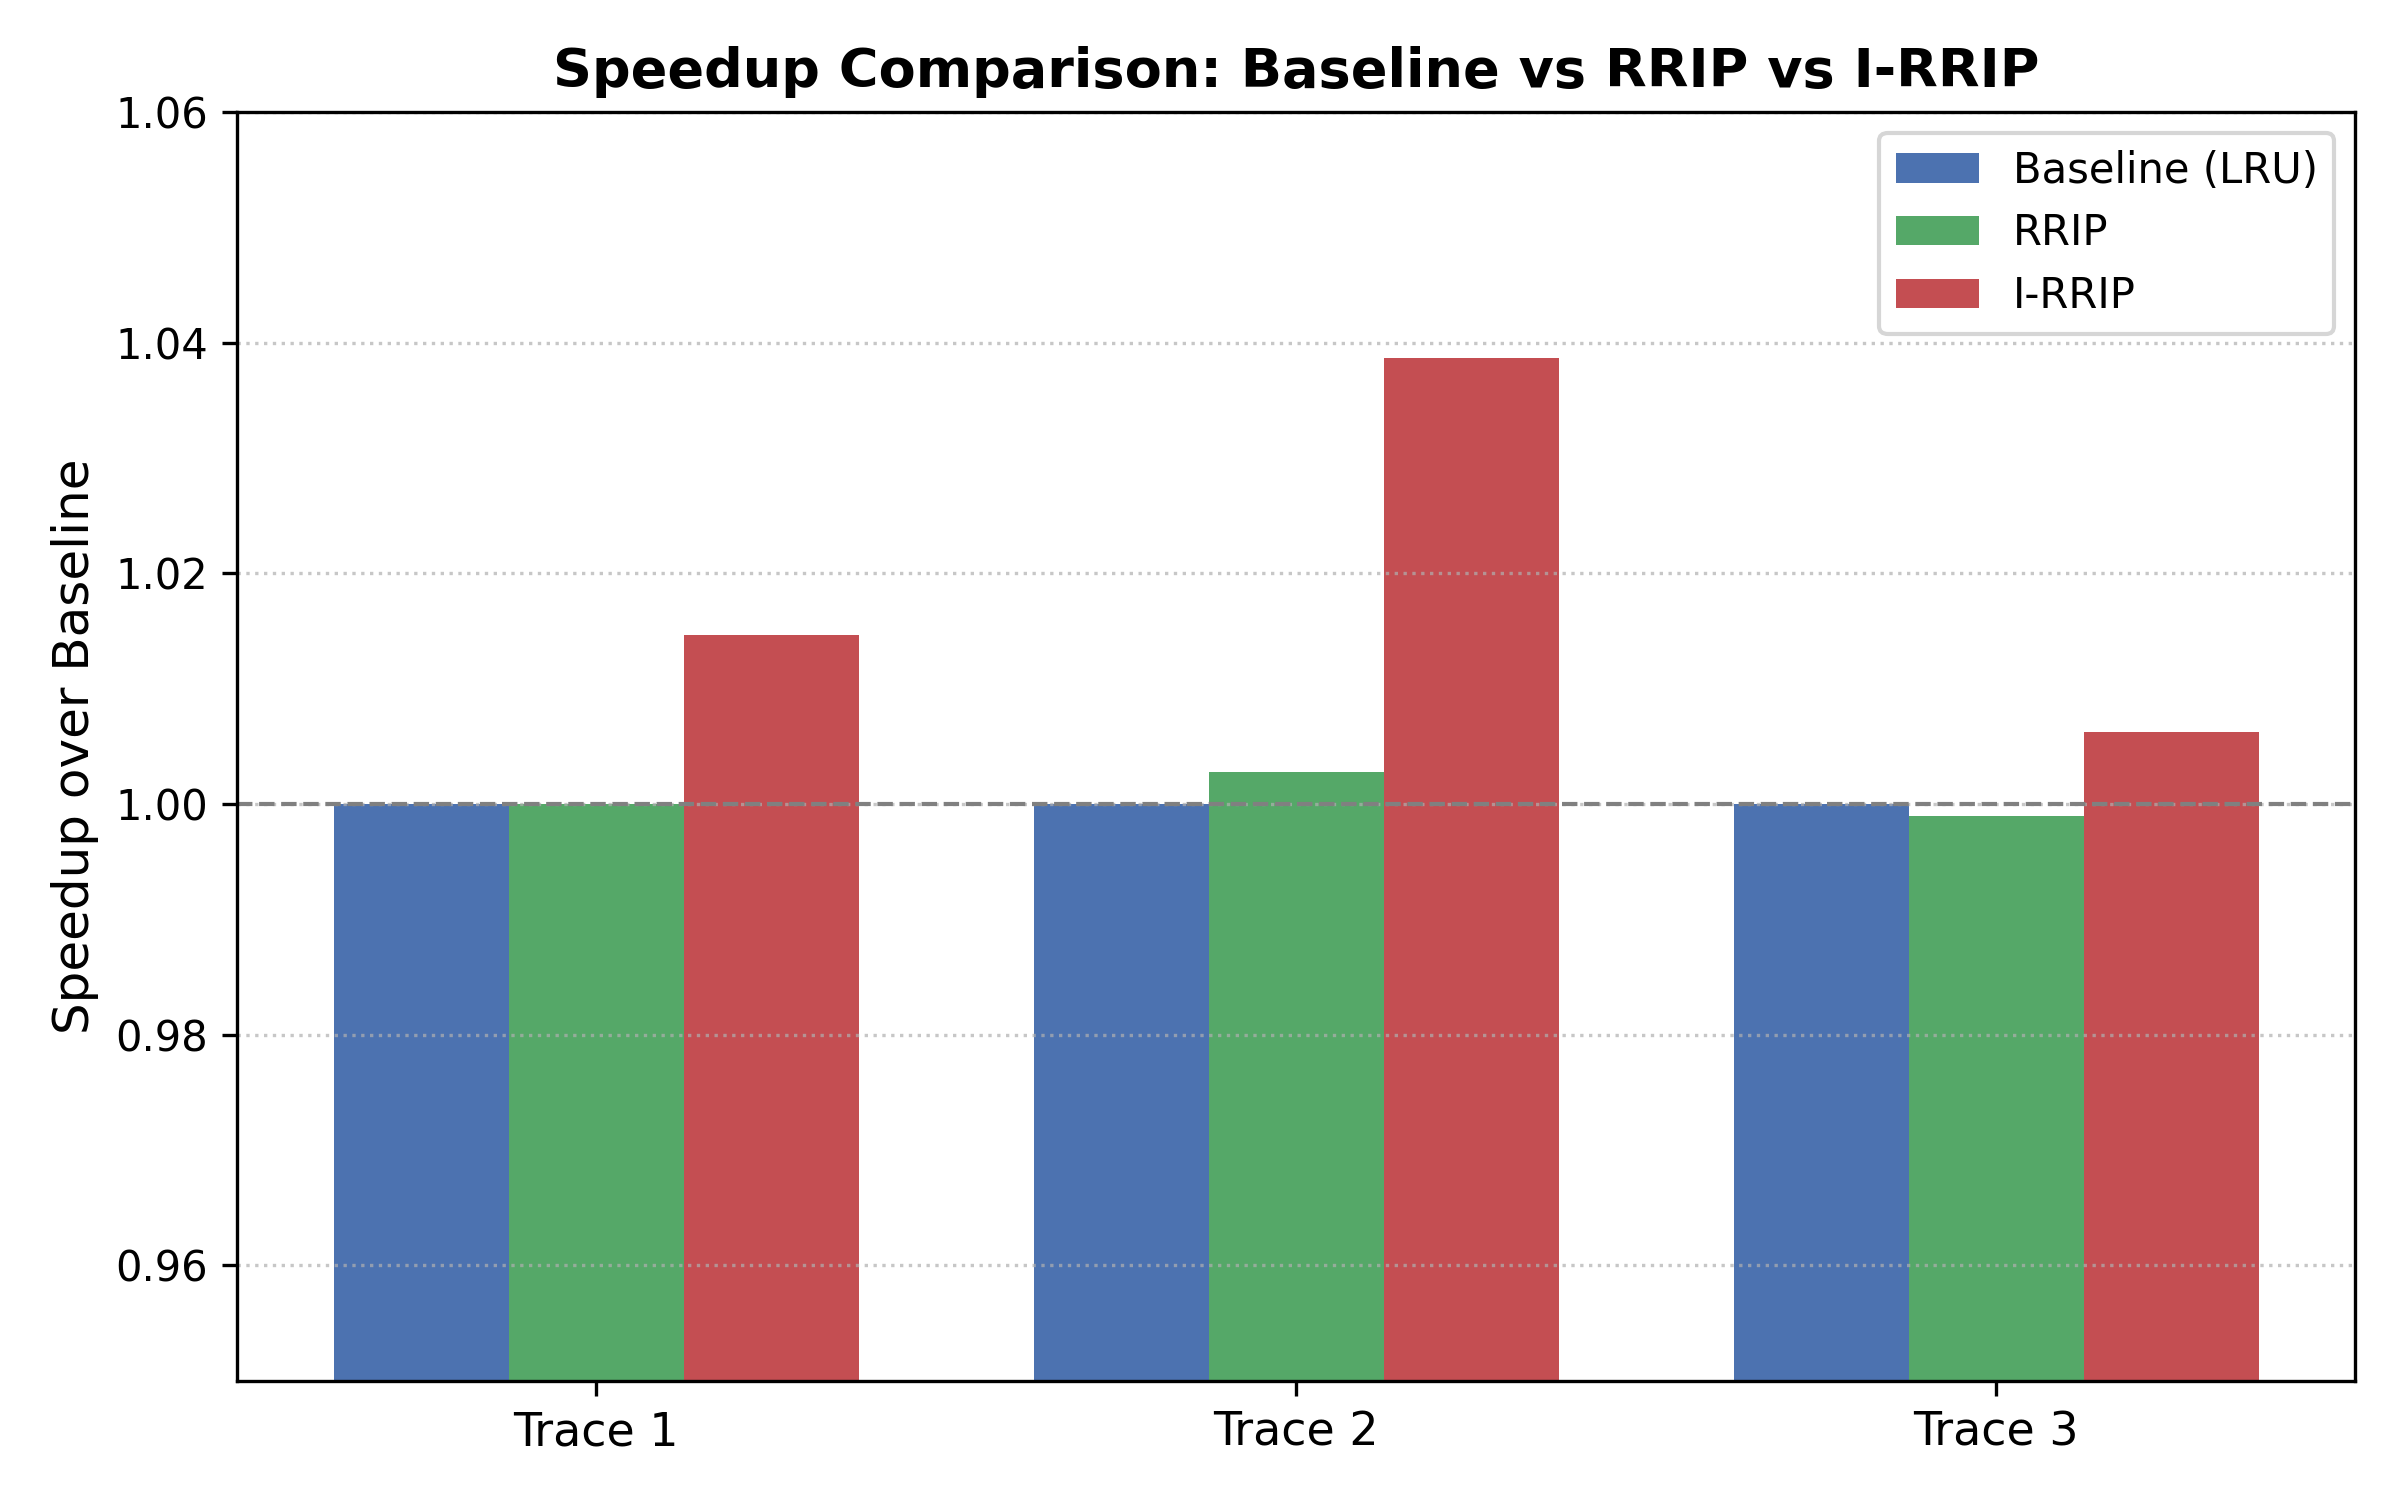
\includegraphics[width=0.85\textwidth]{plots/task2a/task2a_speedup.png}
    \caption{Speedup comparison of Baseline (LRU), RRIP, and I-RRIP across benchmark traces.}
    \label{fig:task2a-speedup}
\end{figure}

\begin{figure}[H]
    \centering
    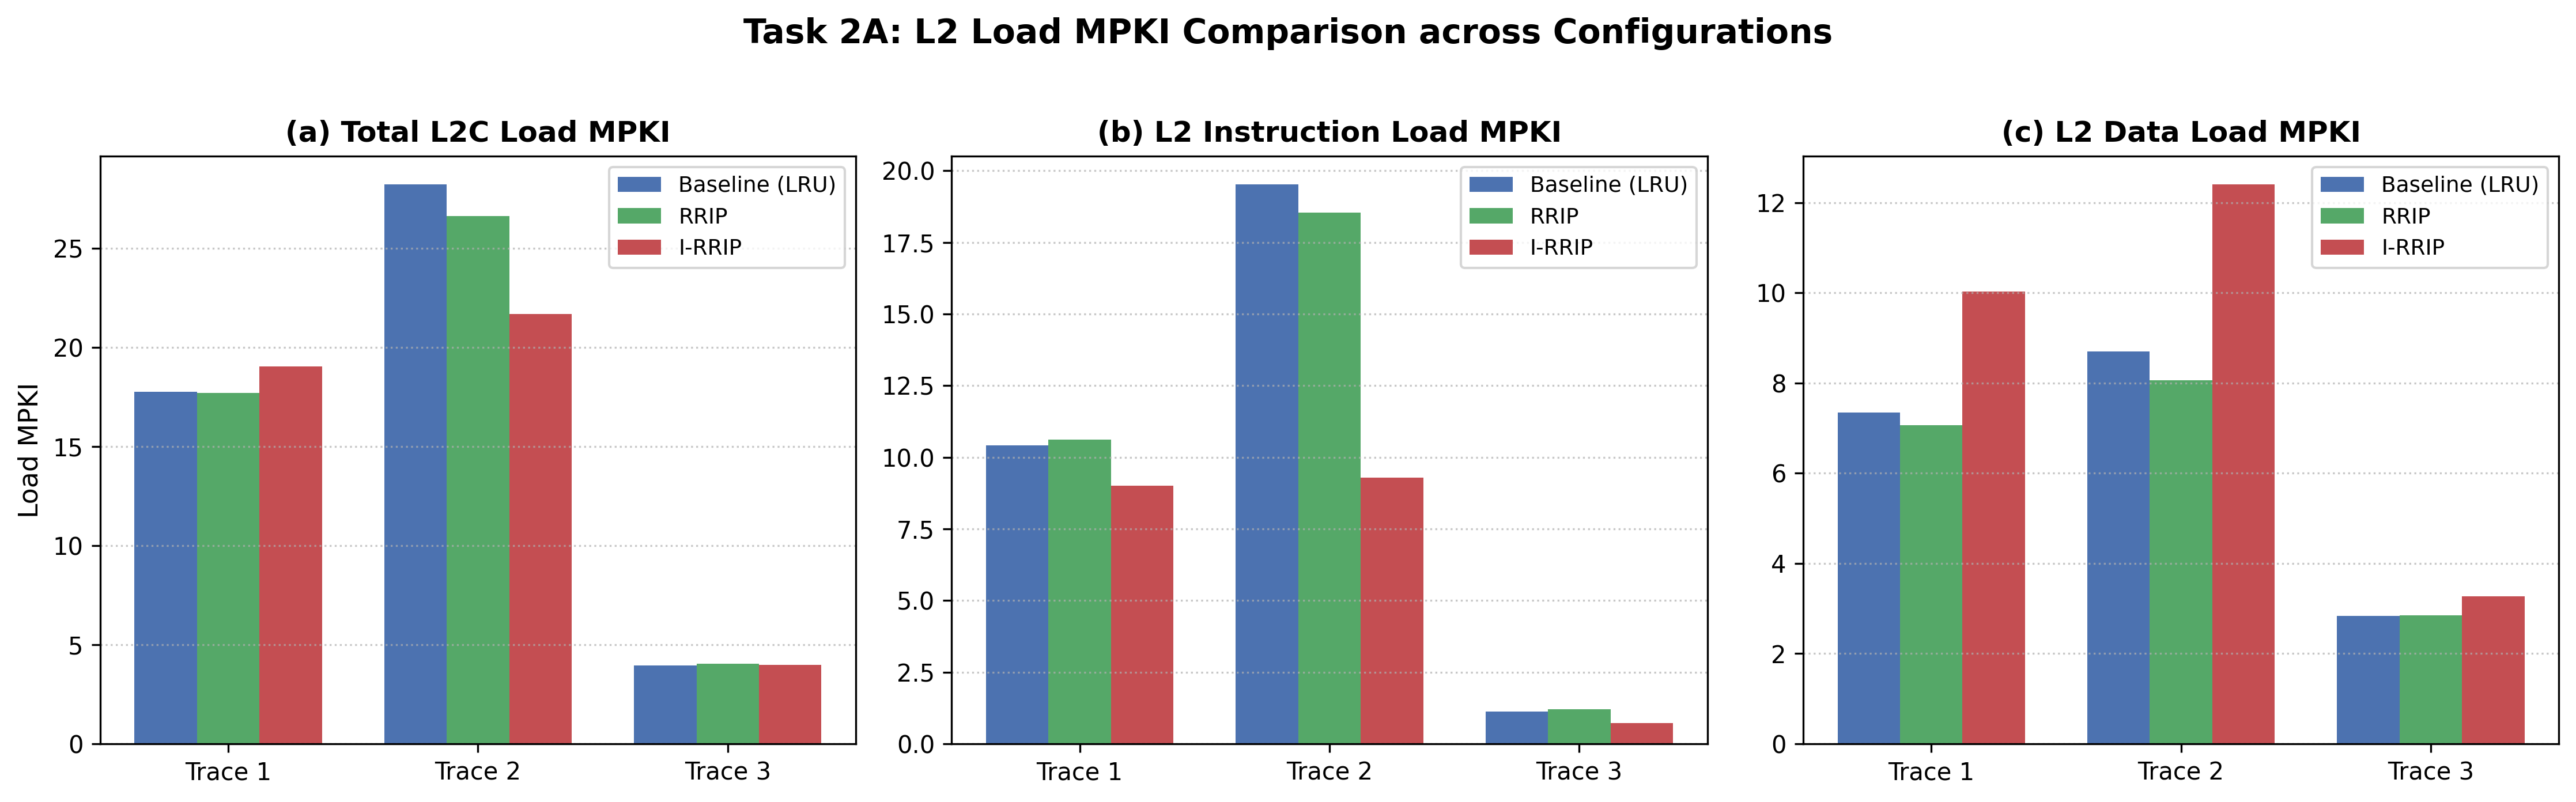
\includegraphics[width=\textwidth]{plots/task2a/task2a_mpki_comparison.png}
    \caption{L2 Load MPKI breakdown for Baseline (LRU), RRIP, and I-RRIP: (a) Total L2C Load MPKI, (b) L2 Instruction Load MPKI, and (c) L2 Data Load MPKI.}
    \label{fig:task2a-mpki}
\end{figure}

\subsubsection{Rationale Behind Insertion Policy}
In standard Static RRIP (SRRIP), all newly filled blocks are inserted with an intermediate prediction value $RRPV = 2$ ($M-1$ in an $M$-bit counter where $M=2$, $\max RRPV = 3$). In I-RRIP, we differentiate between instruction lines and data lines upon insertion:
\begin{itemize}
    \item \textbf{Instruction Lines:} Assigned $RRPV = 1$. By granting instruction lines a lower initial RRPV than data lines, they are placed closer to the MRU state ($RRPV = 0$) and require multiple aging increments before becoming eviction candidates. This provides retention priority, directly protecting instructions from premature eviction.
    \item \textbf{Data Lines:} Assigned $RRPV = 2$. Data lines follow standard distant re-reference prediction, ensuring they do not crowd out instruction lines unless they exhibit repeated temporal reuse.
\end{itemize}

\subsubsection{Rationale Behind Promotion Policy}
Upon a cache hit, both instruction and data lines are promoted directly to $RRPV = 0$ (MRU). Preserving standard hit promotion to 0 guarantees that active working set lines that repeatedly hit remain protected regardless of their type, maintaining high hit rates for frequently accessed data while preventing unnecessary cache thrashing.

\subsubsection{Rationale Behind Eviction Policy}
Standard RRIP chooses the first line with $RRPV = 3$ and increments all lines if none is at $\max RRPV$. In I-RRIP, the eviction policy is instruction-conscious:
\begin{itemize}
    \item \textbf{Primary Candidate Search:} The victim search first targets non-instruction lines that have reached $RRPV = \max RRPV$. If a non-instruction line is found at $RRPV = 3$, it is immediately evicted.
    \item \textbf{Fallback Candidate Search:} If all blocks in the set with $RRPV = 3$ are instruction lines, the policy checks whether \emph{any} non-instruction lines exist in the set. If non-instruction lines exist (even if their RRPV is currently $< 3$), the policy ages all lines (increments RRPV) rather than evicting the instruction line, thereby driving the non-instruction lines toward $RRPV = 3$. Only if a set consists strictly of instruction lines is an instruction line evicted at $RRPV = 3$.
\end{itemize}
This prioritization dramatically cuts instruction misses: on Trace 2, Instruction MPKI drops from 19.53 to 9.28 (a 52.5\% reduction), raising IPC from 0.2506 to 0.2603 (+3.85\% speedup).

\subsection{Dynamic I-RRIP}
\subsubsection{Sensitivity Study of Decision Threshold}

\begin{table}[H]
\centering
\caption{Sensitivity of Dynamic I-RRIP across 5 decision thresholds ($\theta \in \{0.15, 0.20, 0.25, 0.30, 0.35\}$).}
\label{tab:dyn-irrip-threshold}
\resizebox{\textwidth}{!}{
\begin{tabular}{lcccccc}
\toprule
Trace & Threshold ($\theta$) & IPC & Speedup & L2C Load MPKI & L2I Load MPKI & L2D Load MPKI \\
\midrule
Trace 1 & 0.15 & 0.2359 & 1.0156$\times$ & 18.9161 & 9.0097 & 9.9064 \\
Trace 1 & 0.20 & 0.2358 & 1.0149$\times$ & 18.9166 & 9.0107 & 9.9059 \\
Trace 1 & 0.25 & 0.2356 & 1.0143$\times$ & 18.9378 & 9.0335 & 9.9042 \\
Trace 1 & 0.30 & 0.2357 & 1.0148$\times$ & 18.9280 & 9.0256 & 9.9024 \\
Trace 1 & 0.35 & 0.2338 & 1.0066$\times$ & 18.6493 & 9.4235 & 9.2258 \\
\midrule
Trace 2 & 0.15 & 0.2596 & 1.0357$\times$ & 21.2755 & 9.5434 & 11.7321 \\
Trace 2 & 0.20 & 0.2594 & 1.0349$\times$ & 21.3472 & 9.6674 & 11.6799 \\
Trace 2 & 0.25 & 0.2594 & 1.0350$\times$ & 21.4116 & 9.7580 & 11.6536 \\
Trace 2 & 0.30 & 0.2591 & 1.0338$\times$ & 21.5311 & 9.8976 & 11.6334 \\
Trace 2 & 0.35 & 0.2590 & 1.0336$\times$ & 21.6199 & 10.0058 & 11.6141 \\
\midrule
Trace 3 & 0.15 & 0.3825 & 1.0013$\times$ & 4.0512 & 0.9049 & 3.1463 \\
Trace 3 & 0.20 & 0.3824 & 1.0010$\times$ & 4.0504 & 0.9478 & 3.1026 \\
Trace 3 & 0.25 & 0.3823 & 1.0008$\times$ & 4.0617 & 0.9802 & 3.0815 \\
Trace 3 & 0.30 & 0.3824 & 1.0010$\times$ & 4.0524 & 1.0208 & 3.0316 \\
Trace 3 & 0.35 & 0.3825 & 1.0013$\times$ & 4.0578 & 1.0441 & 3.0137 \\
\bottomrule
\end{tabular}
}
\end{table}

\begin{figure}[H]
    \centering
    \begin{subfigure}[b]{0.48\textwidth}
        \centering
        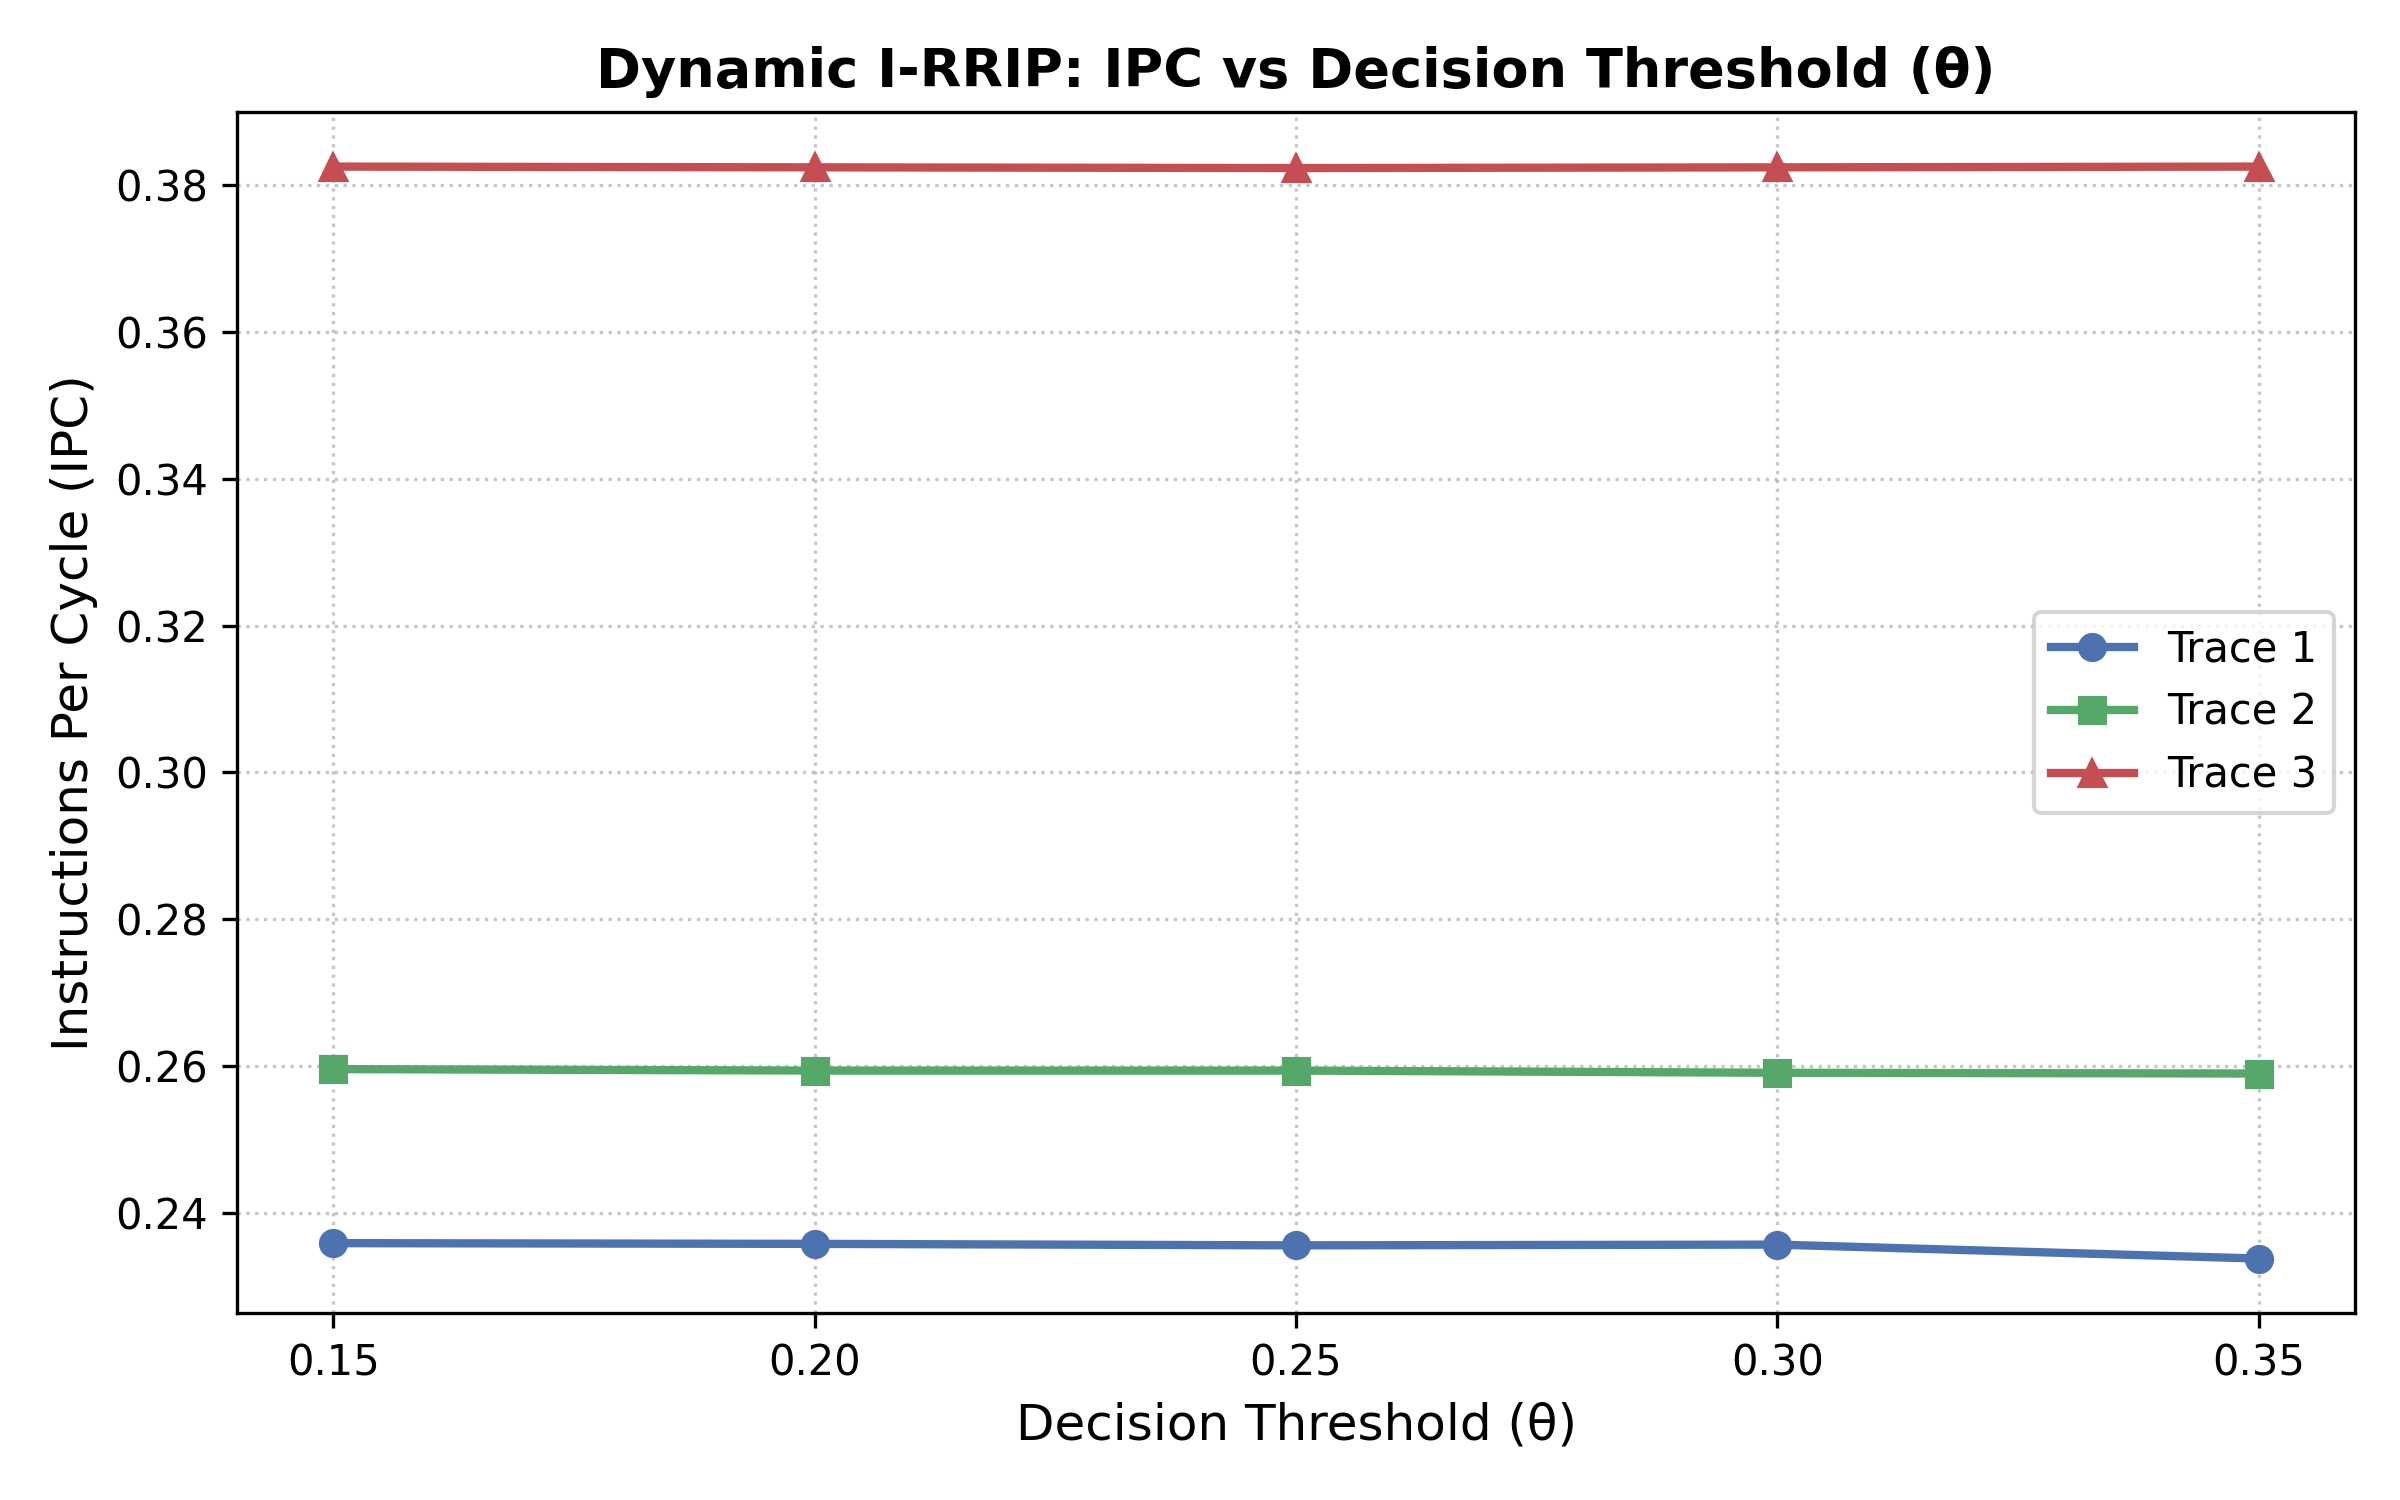
\includegraphics[width=\textwidth]{plots/task2b/task2b_ipc_sensitivity.png}
        \caption{IPC vs Decision Threshold ($\theta$)}
    \end{subfigure}
    \hfill
    \begin{subfigure}[b]{0.48\textwidth}
        \centering
        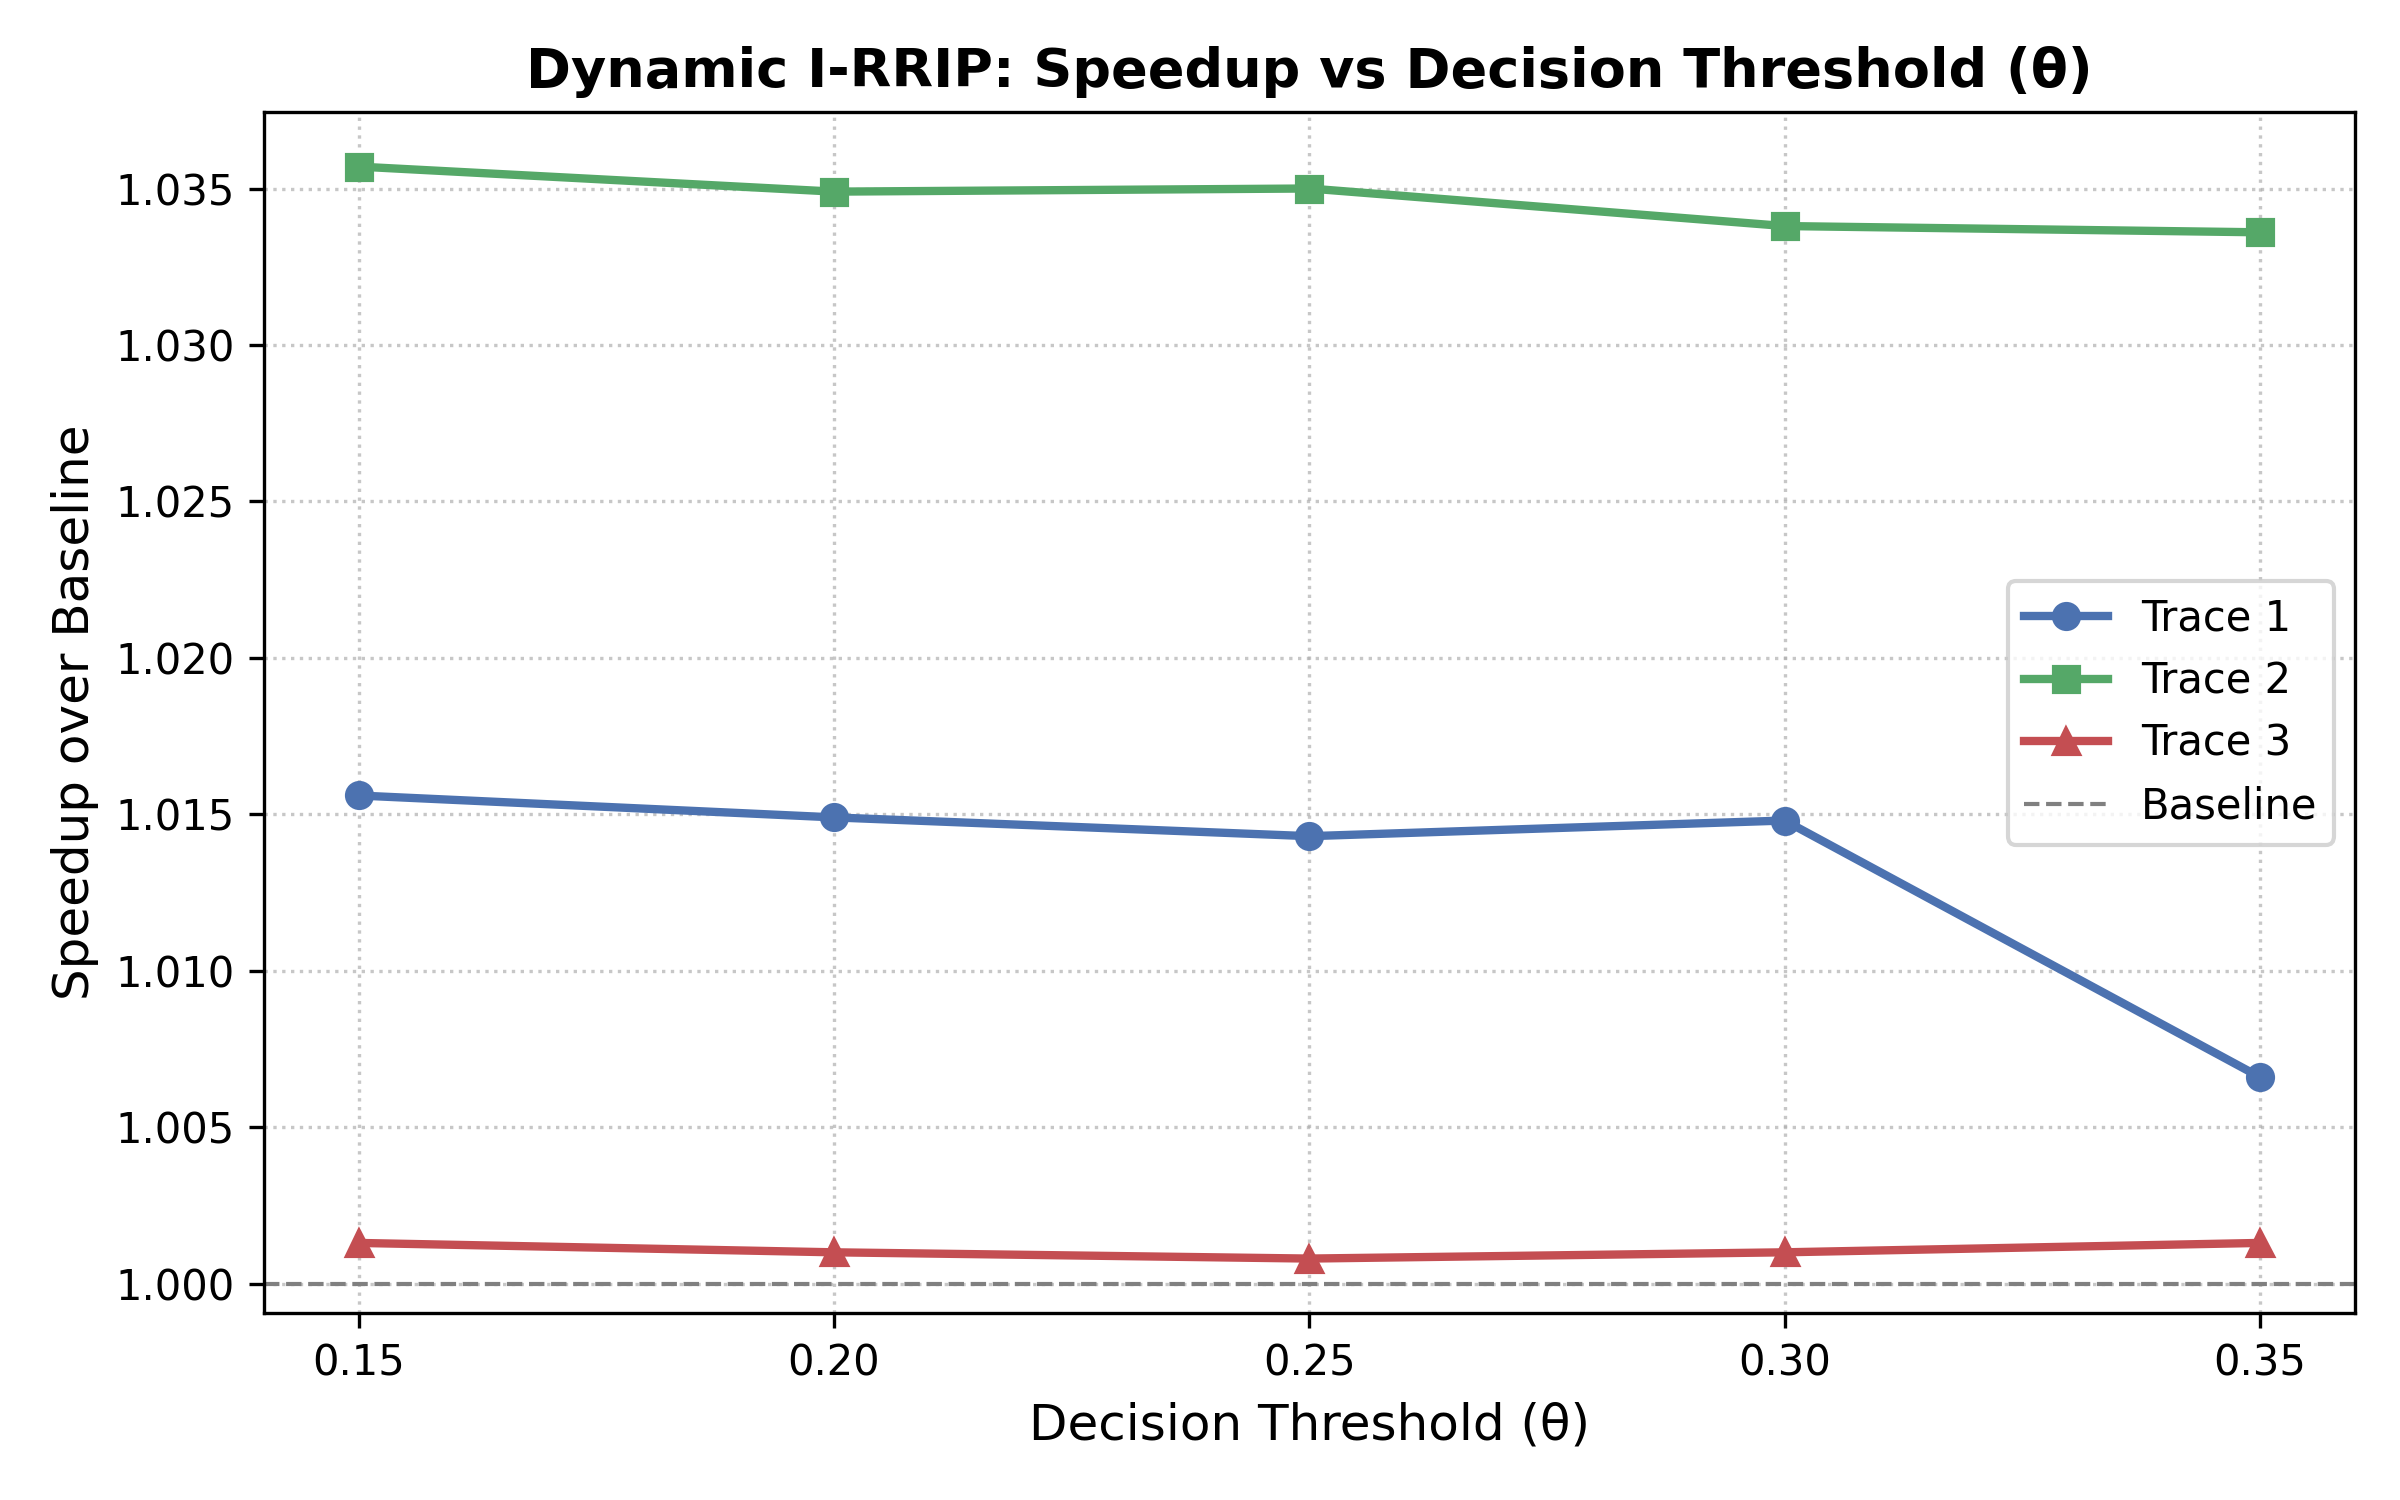
\includegraphics[width=\textwidth]{plots/task2b/task2b_speedup_sensitivity.png}
        \caption{Speedup vs Decision Threshold ($\theta$)}
    \end{subfigure}
    \caption{Performance sensitivity of Dynamic I-RRIP across 5 decision thresholds ($\theta \in \{0.15, 0.20, 0.25, 0.30, 0.35\}$).}
    \label{fig:dyn-irrip-perf-sensitivity}
\end{figure}

\begin{figure}[H]
    \centering
    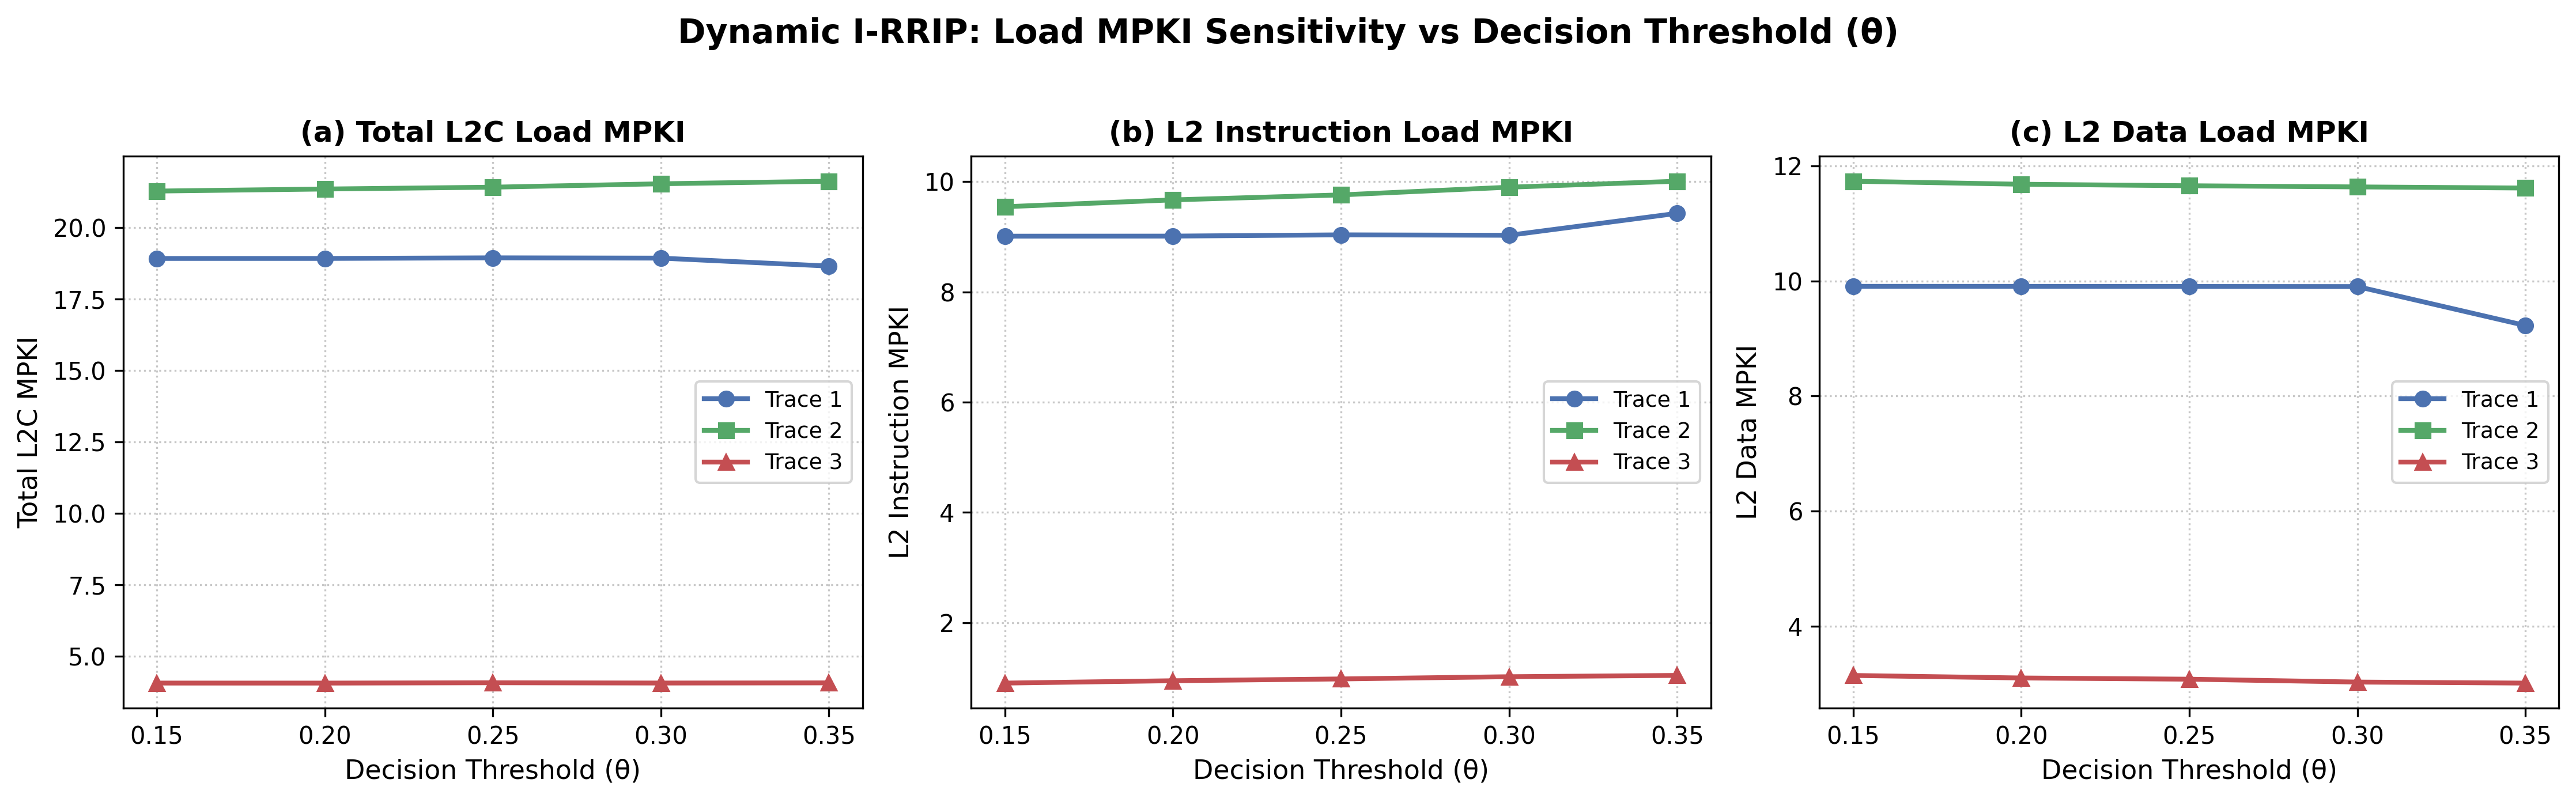
\includegraphics[width=\textwidth]{plots/task2b/task2b_mpki_sensitivity.png}
    \caption{Load MPKI sensitivity of Dynamic I-RRIP across decision thresholds: (a) Total L2C Load MPKI, (b) L2 Instruction Load MPKI, and (c) L2 Data Load MPKI.}
    \label{fig:dyn-irrip-mpki-sensitivity}
\end{figure}

\subsubsection{IPC, Speedup, and Load MPKI Results}

\begin{table}[H]
\centering
\caption{Performance comparison (IPC and Speedup) across Baseline (LRU), RRIP, Static I-RRIP, and Dynamic I-RRIP ($\theta = 0.25$).}
\label{tab:dyn-irrip-performance}
\resizebox{\textwidth}{!}{
\begin{tabular}{lcccccccc}
\toprule
& \multicolumn{4}{c}{IPC} & \multicolumn{4}{c}{Speedup over Baseline} \\
\cmidrule(lr){2-5} \cmidrule(lr){6-9}
Trace & Baseline & RRIP & Static I-RRIP & Dyn I-RRIP & Baseline & RRIP & Static I-RRIP & Dyn I-RRIP \\
\midrule
Trace 1 & 0.2323 & 0.2323 & 0.2357 & 0.2356 & 1.0000$\times$ & 1.0001$\times$ & 1.0148$\times$ & 1.0143$\times$ (+1.43\%) \\
Trace 2 & 0.2506 & 0.2513 & 0.2603 & 0.2594 & 1.0000$\times$ & 1.0026$\times$ & 1.0385$\times$ & 1.0350$\times$ (+3.50\%) \\
Trace 3 & 0.3820 & 0.3816 & 0.3844 & 0.3823 & 1.0000$\times$ & 0.9990$\times$ & 1.0062$\times$ & 1.0008$\times$ (+0.08\%) \\
\bottomrule
\end{tabular}
}
\end{table}

\begin{table}[H]
\centering
\caption{L2 Load MPKI breakdown across all evaluated replacement policies.}
\label{tab:dyn-irrip-mpki}
\begin{tabular}{llccc}
\toprule
Trace & Configuration & L2C Load MPKI & L2 Instruction MPKI & L2 Data MPKI \\
\midrule
Trace 1 & Baseline (LRU)                 & 17.7509 & 10.4030 & 7.3479 \\
        & RRIP                           & 17.6814 & 10.6129 & 7.0684 \\
        & Static I-RRIP                  & 19.0249 & 9.0044  & 10.0204 \\
        & Dynamic I-RRIP ($\theta=0.25$) & 18.9378 & 9.0335  & 9.9042 \\
\midrule
Trace 2 & Baseline (LRU)                 & 28.2286 & 19.5298 & 8.6988 \\
        & RRIP                           & 26.6066 & 18.5456 & 8.0610 \\
        & Static I-RRIP                  & 21.6864 & 9.2780  & 12.4084 \\
        & Dynamic I-RRIP ($\theta=0.25$) & 21.4116 & 9.7580  & 11.6536 \\
\midrule
Trace 3 & Baseline (LRU)                 & 3.9592  & 1.1232  & 2.8360 \\
        & RRIP                           & 4.0443  & 1.1976  & 2.8467 \\
        & Static I-RRIP                  & 3.9884  & 0.7153  & 3.2731 \\
        & Dynamic I-RRIP ($\theta=0.25$) & 4.0617  & 0.9802  & 3.0815 \\
\bottomrule
\end{tabular}
\end{table}

\begin{figure}[H]
    \centering
    \begin{subfigure}[b]{0.48\textwidth}
        \centering
        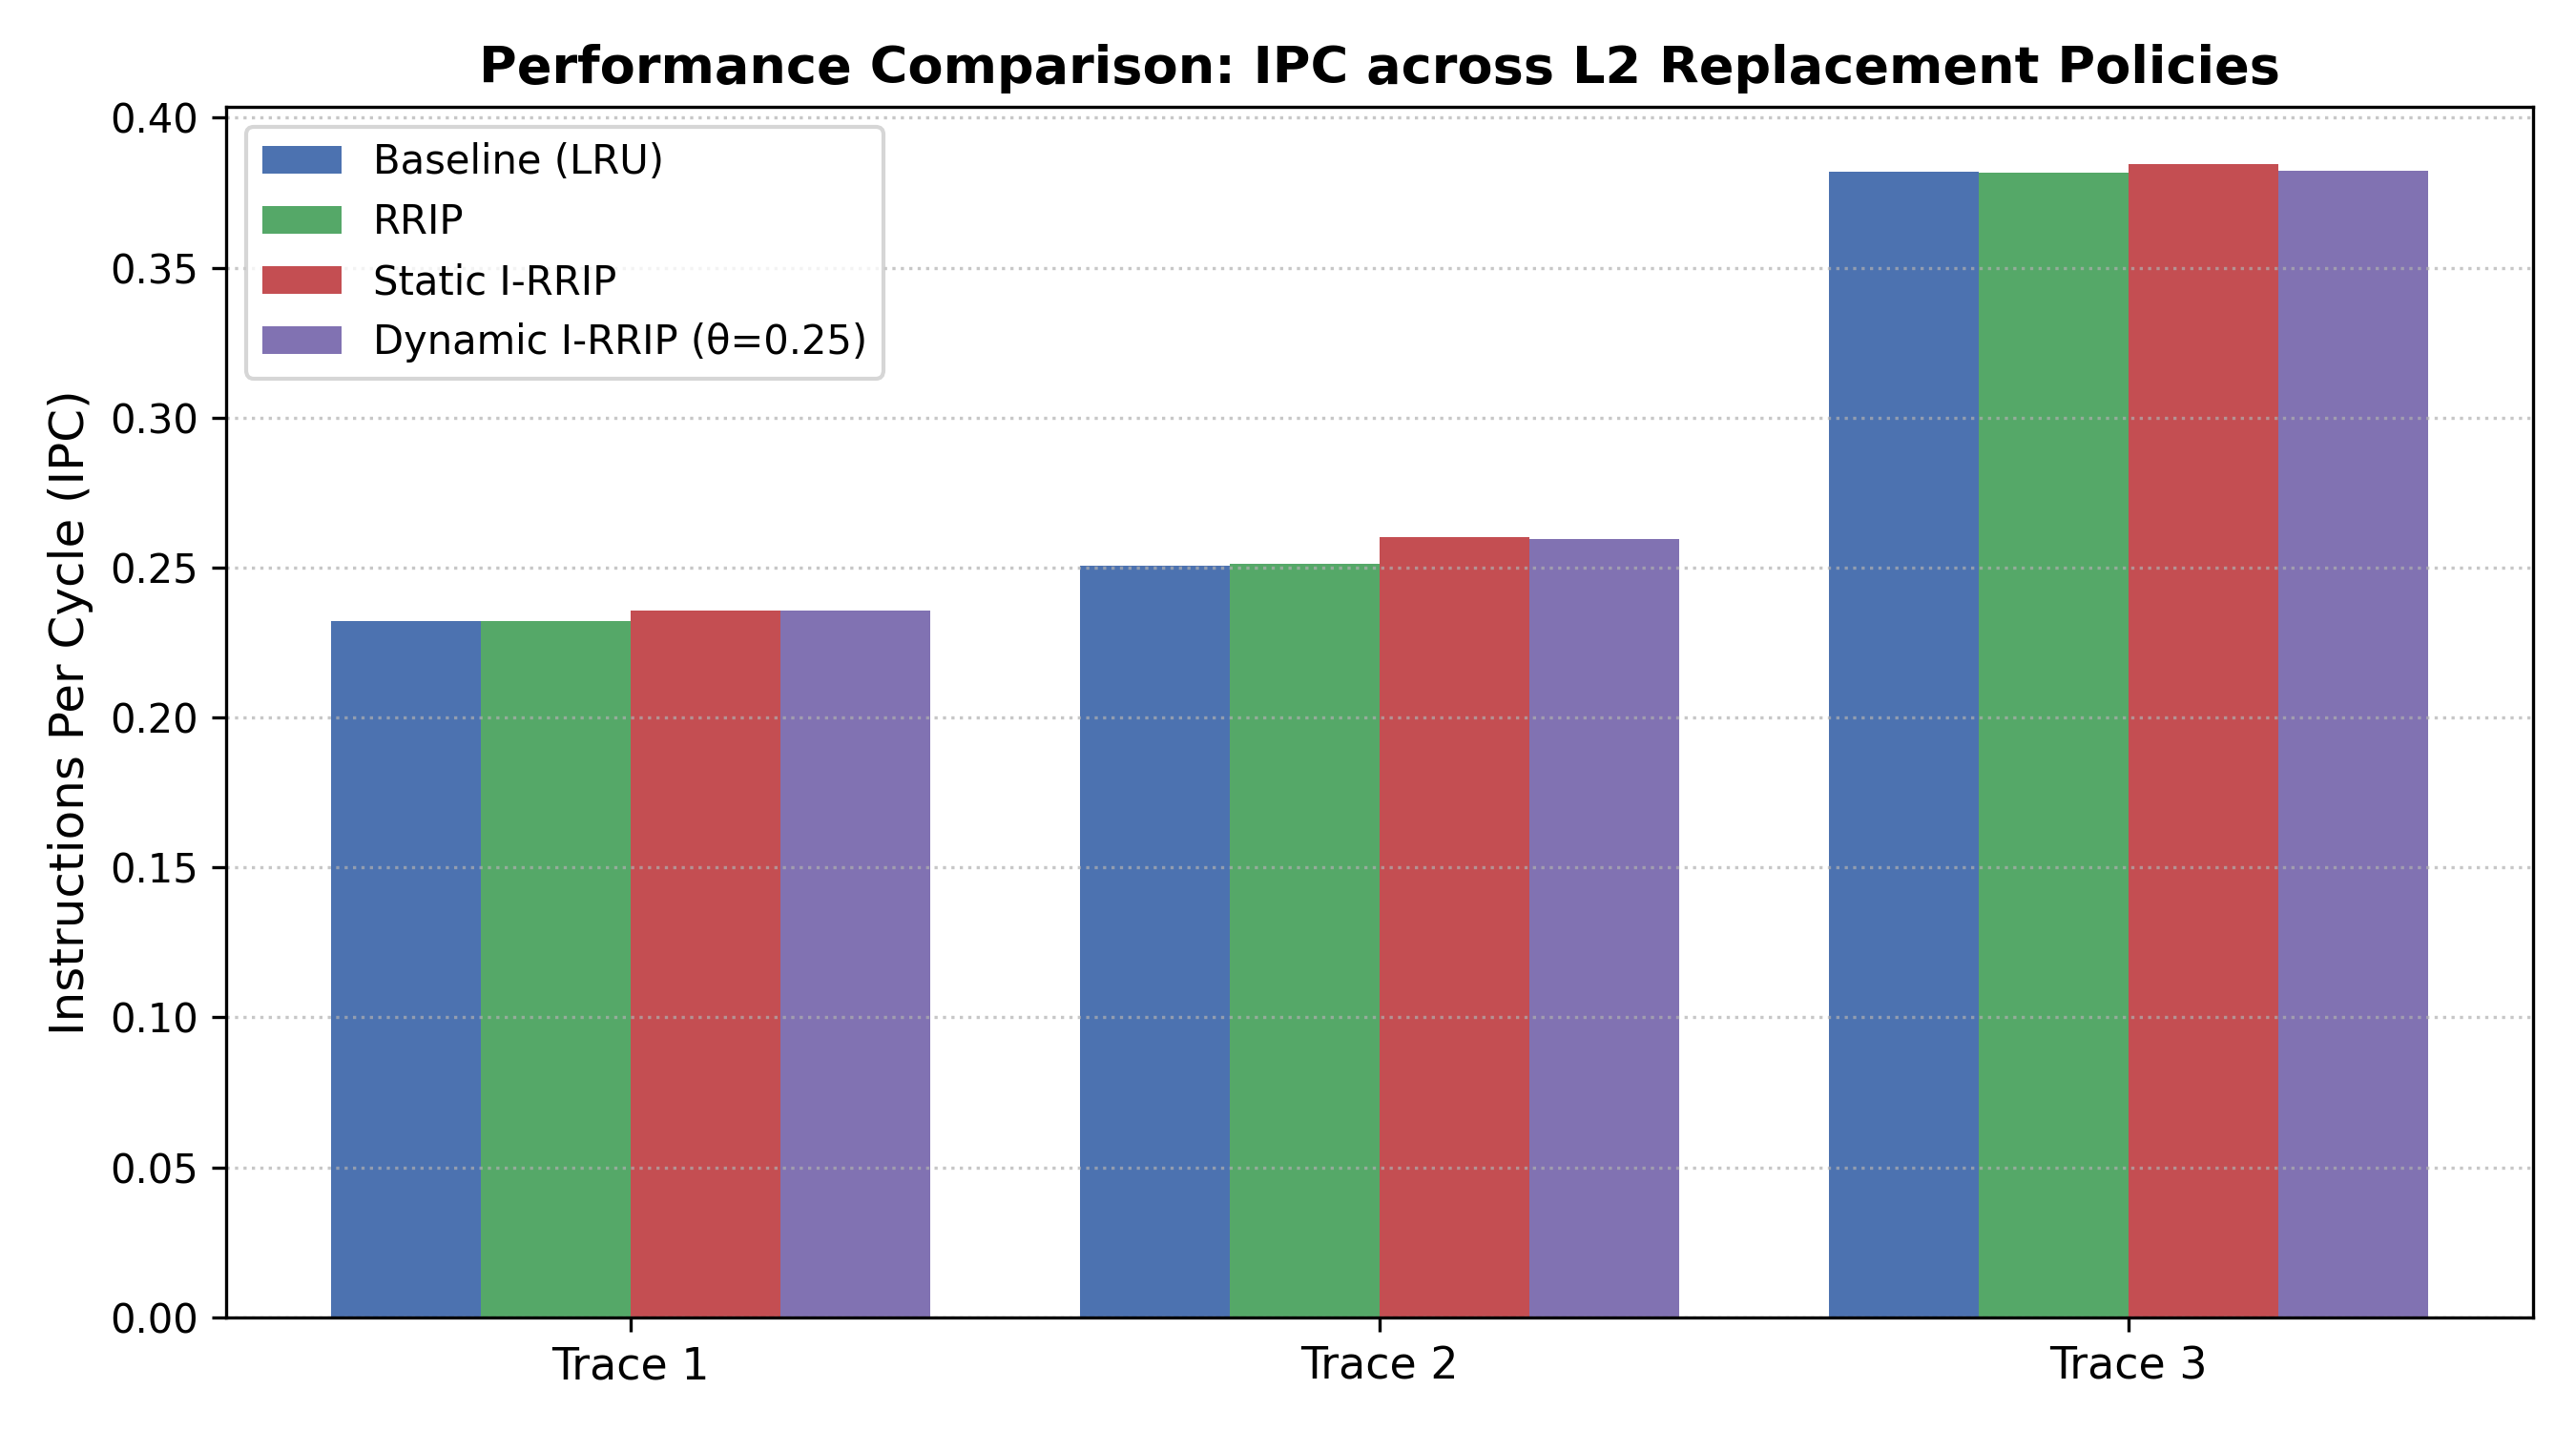
\includegraphics[width=\textwidth]{plots/task2b/task2b_ipc_comparison.png}
        \caption{IPC Comparison}
    \end{subfigure}
    \hfill
    \begin{subfigure}[b]{0.48\textwidth}
        \centering
        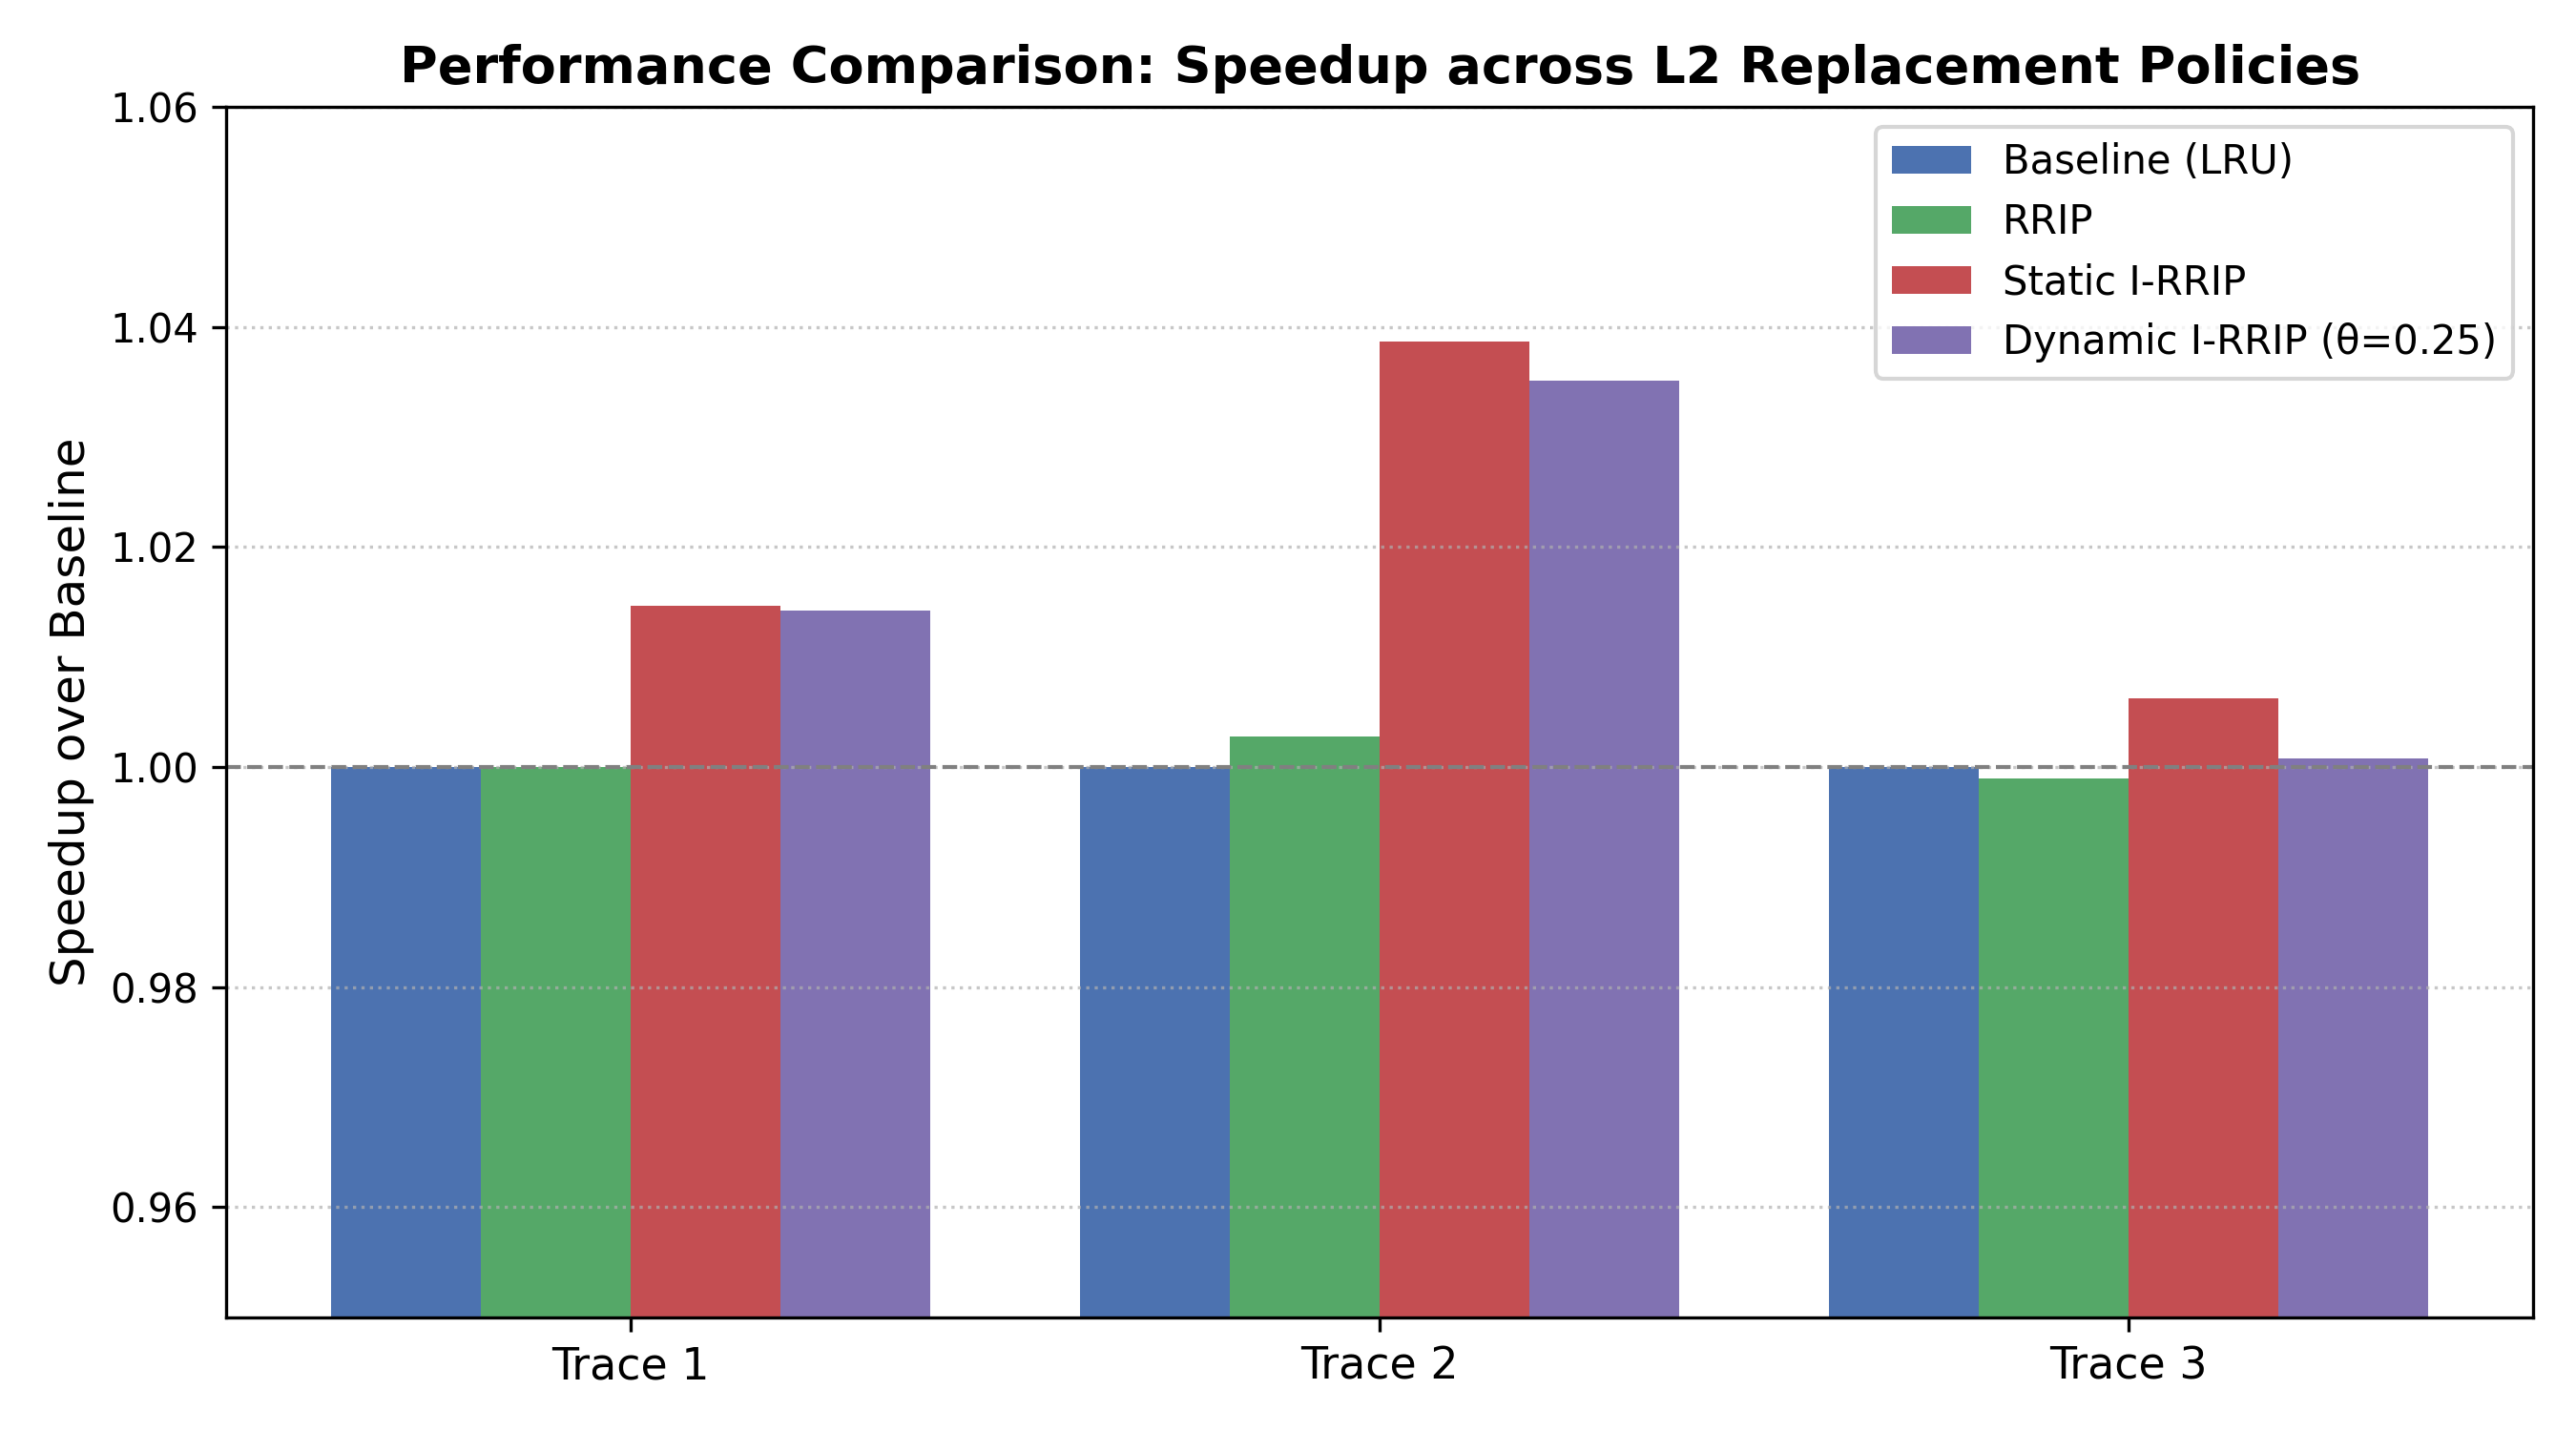
\includegraphics[width=\textwidth]{plots/task2b/task2b_speedup_comparison.png}
        \caption{Speedup Comparison}
    \end{subfigure}
    \caption{Performance comparison (IPC and Speedup) across Baseline (LRU), RRIP, Static I-RRIP, and Dynamic I-RRIP ($\theta = 0.25$).}
    \label{fig:dyn-irrip-perf-comparison}
\end{figure}

\begin{figure}[H]
    \centering
    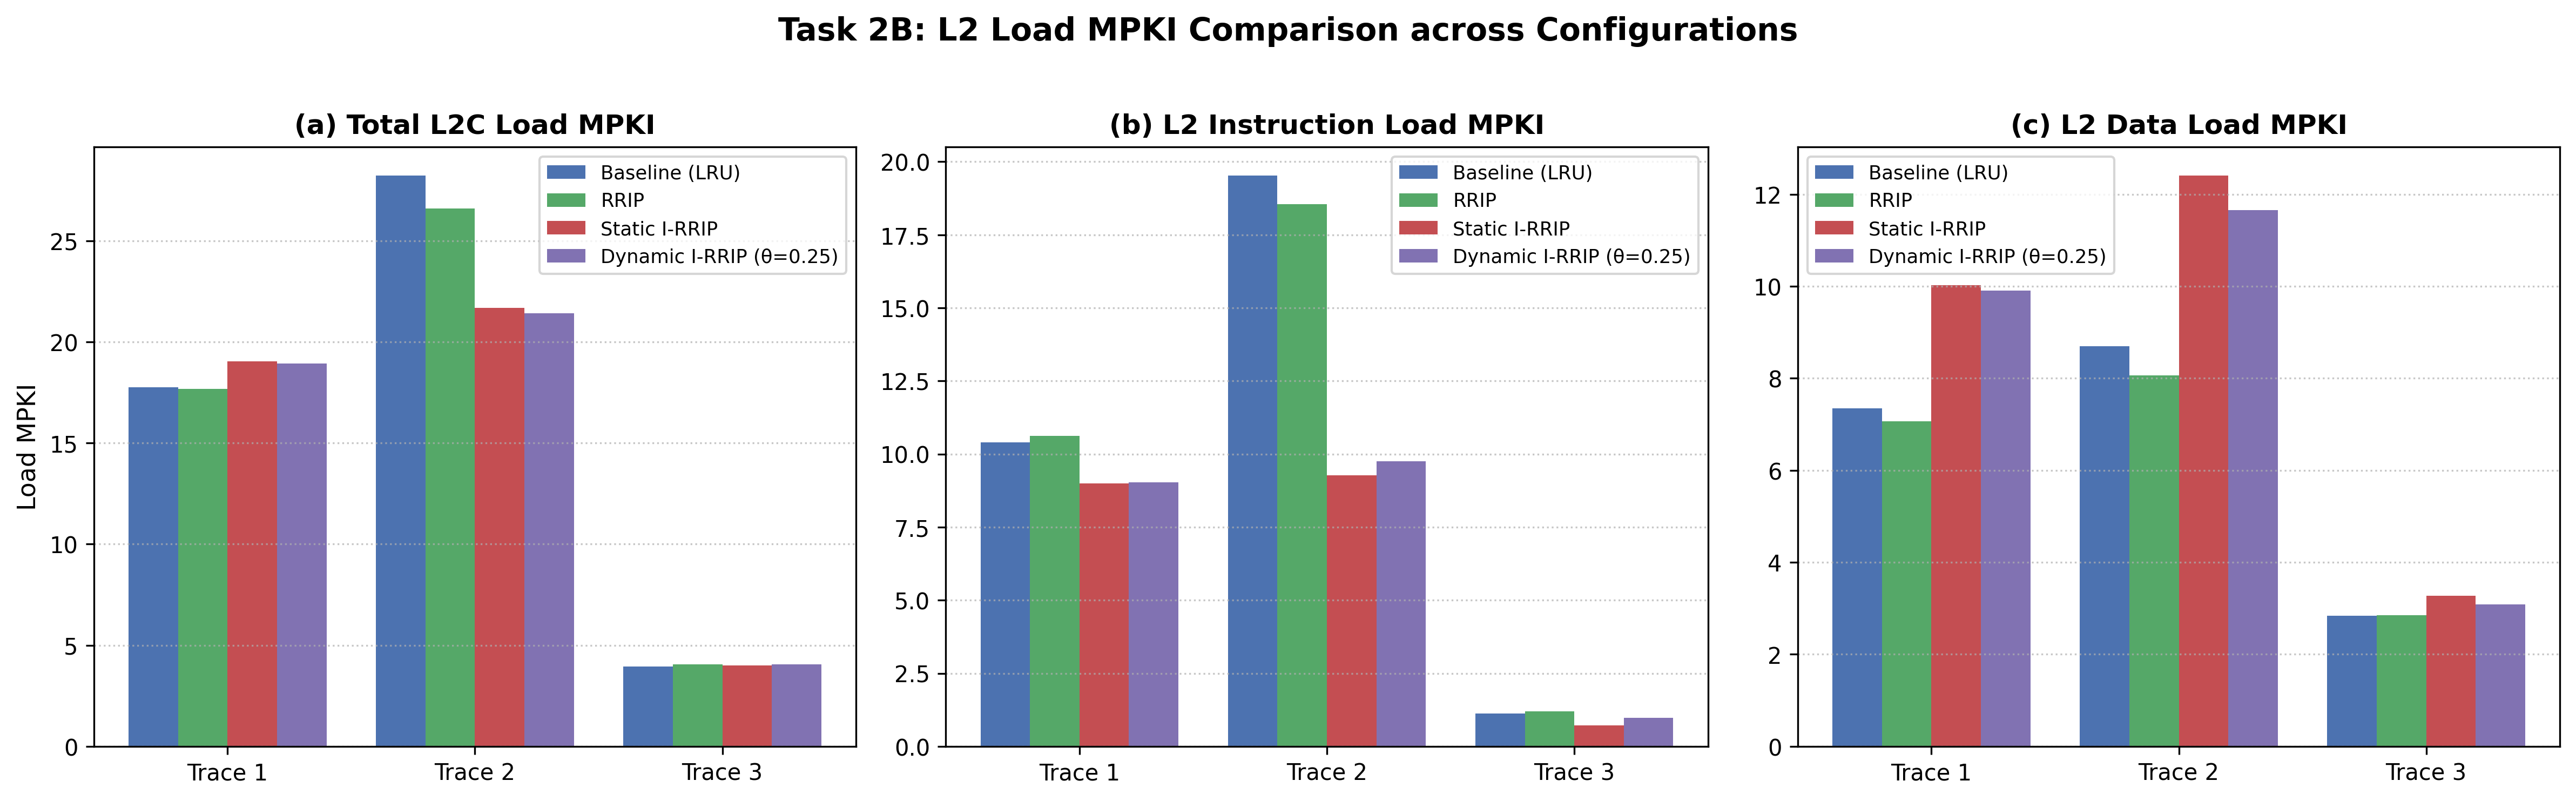
\includegraphics[width=\textwidth]{plots/task2b/task2b_mpki_comparison.png}
    \caption{L2 Load MPKI breakdown across Baseline (LRU), RRIP, Static I-RRIP, and Dynamic I-RRIP ($\theta = 0.25$): (a) Total L2C Load MPKI, (b) L2 Instruction Load MPKI, and (c) L2 Data Load MPKI.}
    \label{fig:dyn-irrip-mpki-comparison}
\end{figure}

\subsubsection{Rationale for the Number of Leader Sets and Decision Logic}
\begin{itemize}
    \item \textbf{Number of Leader Sets:} ChampSim's L2 cache contains 1024 sets. We designate 32 leader sets distributed uniformly using modular indexing ($\text{set} \pmod{32} == 0$), which corresponds to exactly $32/1024 = 3.125\%$ (or 1 in 32 sets) of the cache. As demonstrated in classic set-dueling literature (Qureshi et al., ISCA 2006), 32 sampled sets provide statistically significant representation of total workload cache behavior across diverse access patterns while bounding the penalty of suboptimal leader sets to less than $3.2\%$.
    \item \textbf{Dedicated Leader Set Operation:} The 32 leader sets unconditionally run standard RRIP. They track four hardware counters: $\text{leader\_instr\_access}$, $\text{leader\_instr\_miss}$, $\text{leader\_total\_access}$, and $\text{leader\_total\_miss}$.
    \item \textbf{Decision Formula:} The follower sets query the sampled instruction intensity ratio:
    \begin{equation}
        \text{Ratio} = \frac{\text{leader\_instr\_access} + \text{leader\_instr\_miss}}{\text{leader\_total\_access} + \text{leader\_total\_miss}}
    \end{equation}
    If $\text{Ratio} > \theta$, the follower sets operate in I-RRIP mode (prioritizing instruction lines in insertion and eviction). When $\text{Ratio} \le \theta$, follower sets fall back to standard RRIP mode.
    \item \textbf{Dynamic Phase Tracking and Aging:} To allow the policy to adapt rapidly to application phase changes and prevent counter saturation, all four leader counters are halved (right-shifted by 1) whenever $\text{leader\_total\_access}$ reaches an epoch of 4096 accesses. This decaying window prevents stale execution history from dominating future replacement decisions.
    \item \textbf{Threshold Sensitivity Analysis:}
    As seen in Table~\ref{tab:dyn-irrip-threshold} and Figures~\ref{fig:dyn-irrip-perf-sensitivity} and~\ref{fig:dyn-irrip-mpki-sensitivity}, lower thresholds ($\theta = 0.15, 0.20$) allow follower sets to activate I-RRIP aggressively, yielding maximum instruction miss reduction (Trace 2 Instr MPKI drops from 18.55 down to 9.54, giving 1.0357$\times$ speedup). As the threshold is increased to 0.35, the policy becomes more conservative, falling back to RRIP more often, which slightly raises instruction MPKI but curtails data miss increases (on Trace 1, Data MPKI drops from 9.91 to 9.22). Threshold $\theta = 0.25$ provides an ideal balance across workloads.
\end{itemize}


\section{Data Prefetcher + Cache Replacement Policy}
\subsection{Incorporating SPP with Dynamic I-RRIP}
\subsubsection{IPC, Speedup, Prefetch Accuracy, Coverage, and Load MPKI Results}

\begin{table}[H]
\centering
\caption{Performance comparison of Baseline, SPP, Dynamic I-RRIP, and SPP with Dynamic I-RRIP across benchmark traces.}
\label{tab:task3-performance}
\resizebox{\textwidth}{!}{
\begin{tabular}{llcccccccc}
\toprule
Trace & Configuration & IPC & Speedup & Accuracy & Coverage & L1D MPKI & L2C MPKI & L2I MPKI & L2D MPKI \\
\midrule
Trace 1 & Baseline & 0.2321 & 1.0000$\times$ & -- & -- & 10.6788 & 17.7251 & 10.3665 & 7.3586 \\
        & SPP & 0.2338 & 1.0073$\times$ & 53.48\% & 9.26\% & 9.6901 & 16.9386 & 10.4200 & 6.5186 \\
        & Dynamic I-RRIP & 0.2324 & 1.0014$\times$ & -- & -- & 10.6789 & 17.4772 & 10.2429 & 7.2343 \\
        & \textbf{SPP + Dynamic I-RRIP} & \textbf{0.2343} & \textbf{1.0092$\times$} & 53.53\% & 9.26\% & 9.6902 & 16.6096 & 10.2223 & 6.3873 \\
\midrule
Trace 2 & Baseline & 0.2500 & 1.0000$\times$ & -- & -- & 13.5372 & 28.5496 & 19.8440 & 8.7056 \\
        & SPP & 0.2511 & 1.0046$\times$ & 46.03\% & 2.45\% & 13.2056 & 28.4368 & 20.0366 & 8.4002 \\
        & Dynamic I-RRIP & 0.2550 & 1.0201$\times$ & -- & -- & 13.5413 & 23.7324 & 14.6092 & 9.1232 \\
        & \textbf{SPP + Dynamic I-RRIP} & \textbf{0.2564} & \textbf{1.0255$\times$} & 45.34\% & 2.38\% & 13.2157 & 23.4646 & 14.6674 & 8.7972 \\
\midrule
Trace 3 & Baseline & 0.3819 & 1.0000$\times$ & -- & -- & 3.4036 & 3.9612 & 1.1265 & 2.8347 \\
        & SPP & 0.3883 & 1.0168$\times$ & 44.96\% & 14.37\% & 2.9145 & 3.3203 & 1.1435 & 2.1768 \\
        & Dynamic I-RRIP & 0.3818 & 0.9998$\times$ & -- & -- & 3.4037 & 3.9112 & 1.0898 & 2.8214 \\
        & \textbf{SPP + Dynamic I-RRIP} & \textbf{0.3884} & \textbf{1.0172$\times$} & 44.96\% & 14.45\% & 2.9116 & 3.2278 & 1.0792 & 2.1486 \\
\bottomrule
\end{tabular}
}
\end{table}

\begin{figure}[H]
    \centering
    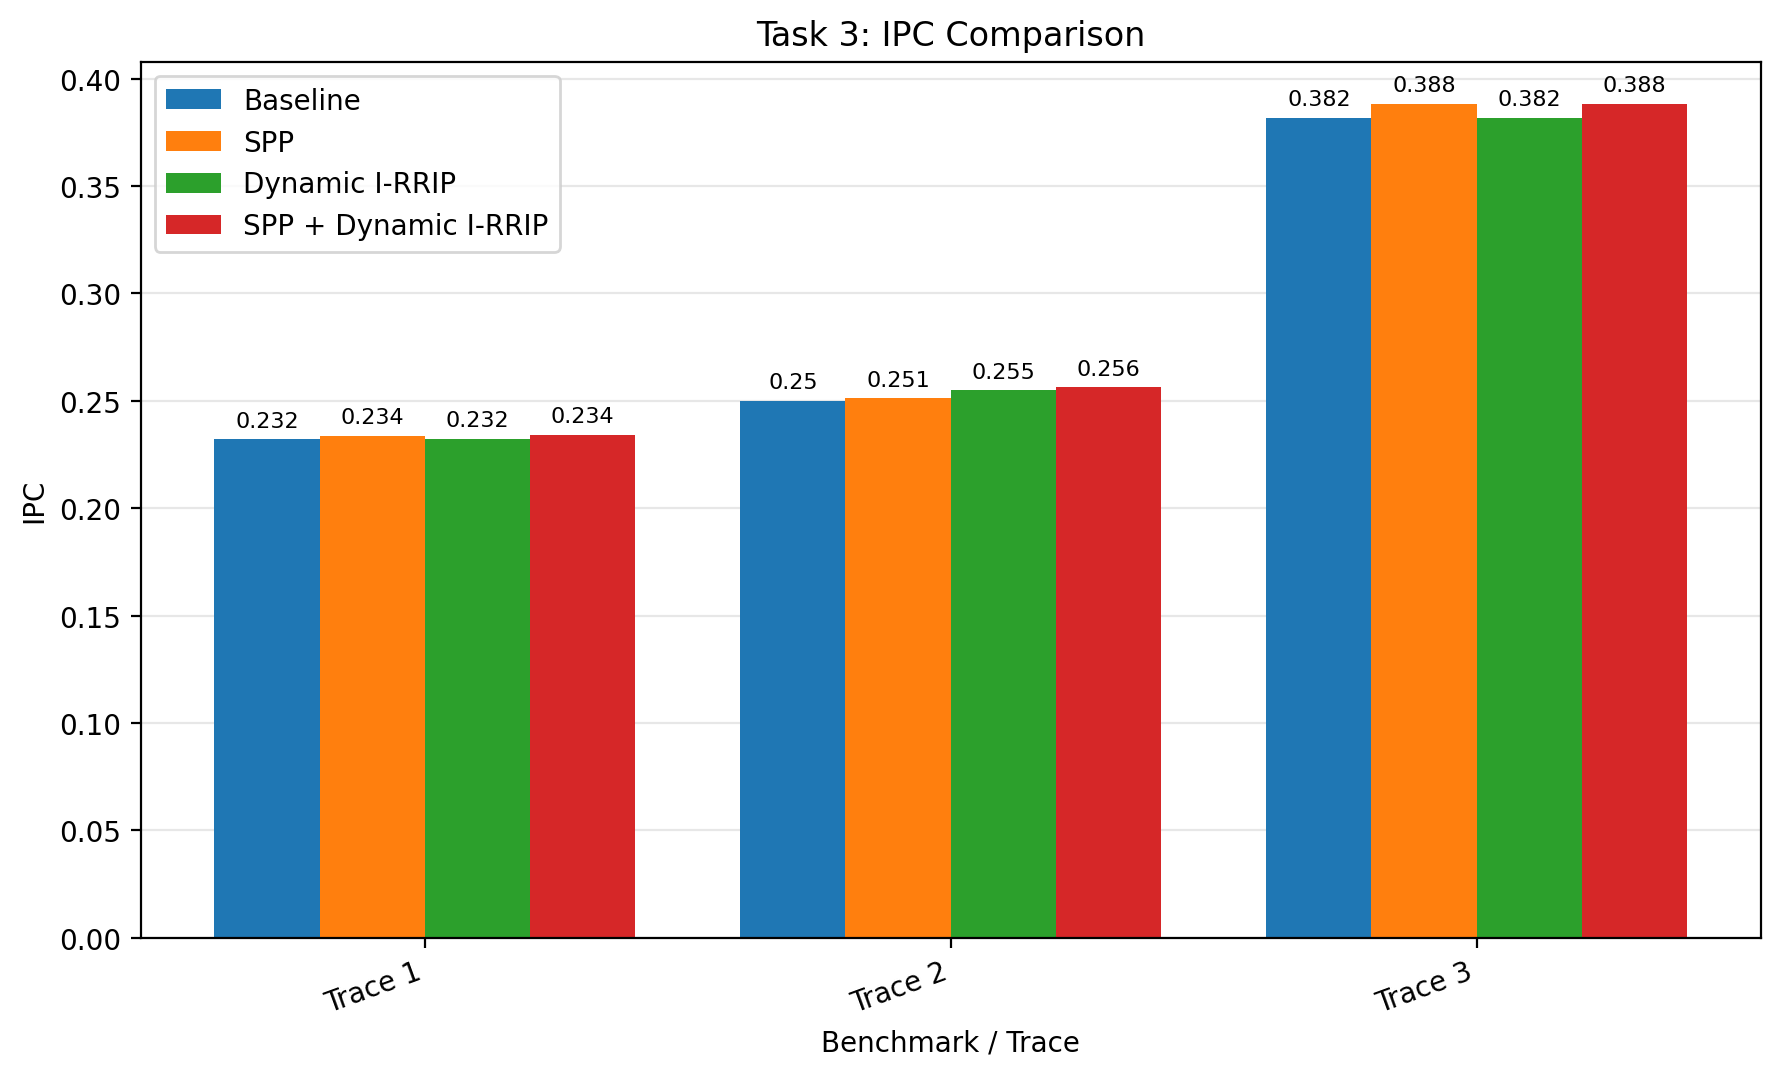
\includegraphics[width=0.85\textwidth]{task3_ipc.png}
    \caption{IPC comparison across Baseline, SPP, Dynamic I-RRIP, and combined SPP + Dynamic I-RRIP.}
    \label{fig:task3-ipc}
\end{figure}

\begin{figure}[H]
    \centering
    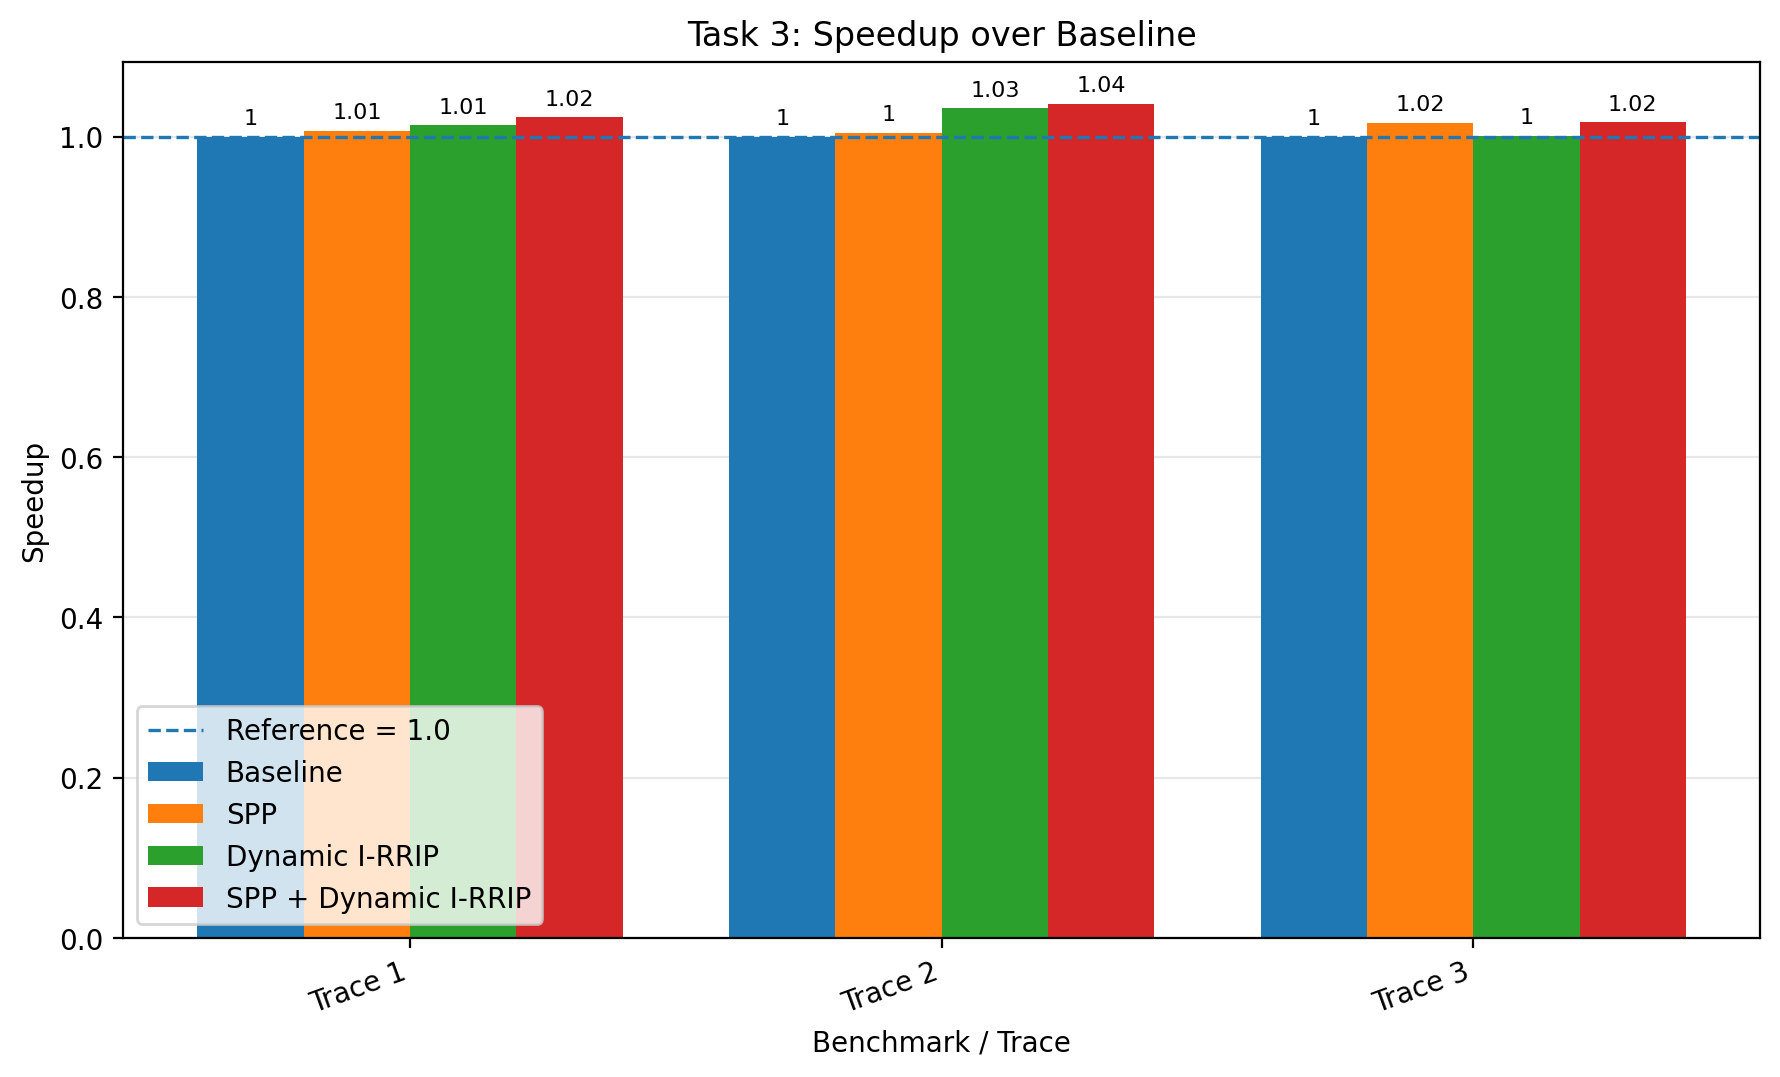
\includegraphics[width=0.85\textwidth]{task3_speedup.png}
    \caption{Speedup comparison over Baseline across configurations.}
    \label{fig:task3-speedup}
\end{figure}

\begin{figure}[H]
    \centering
    \begin{subfigure}[b]{0.48\textwidth}
        \centering
        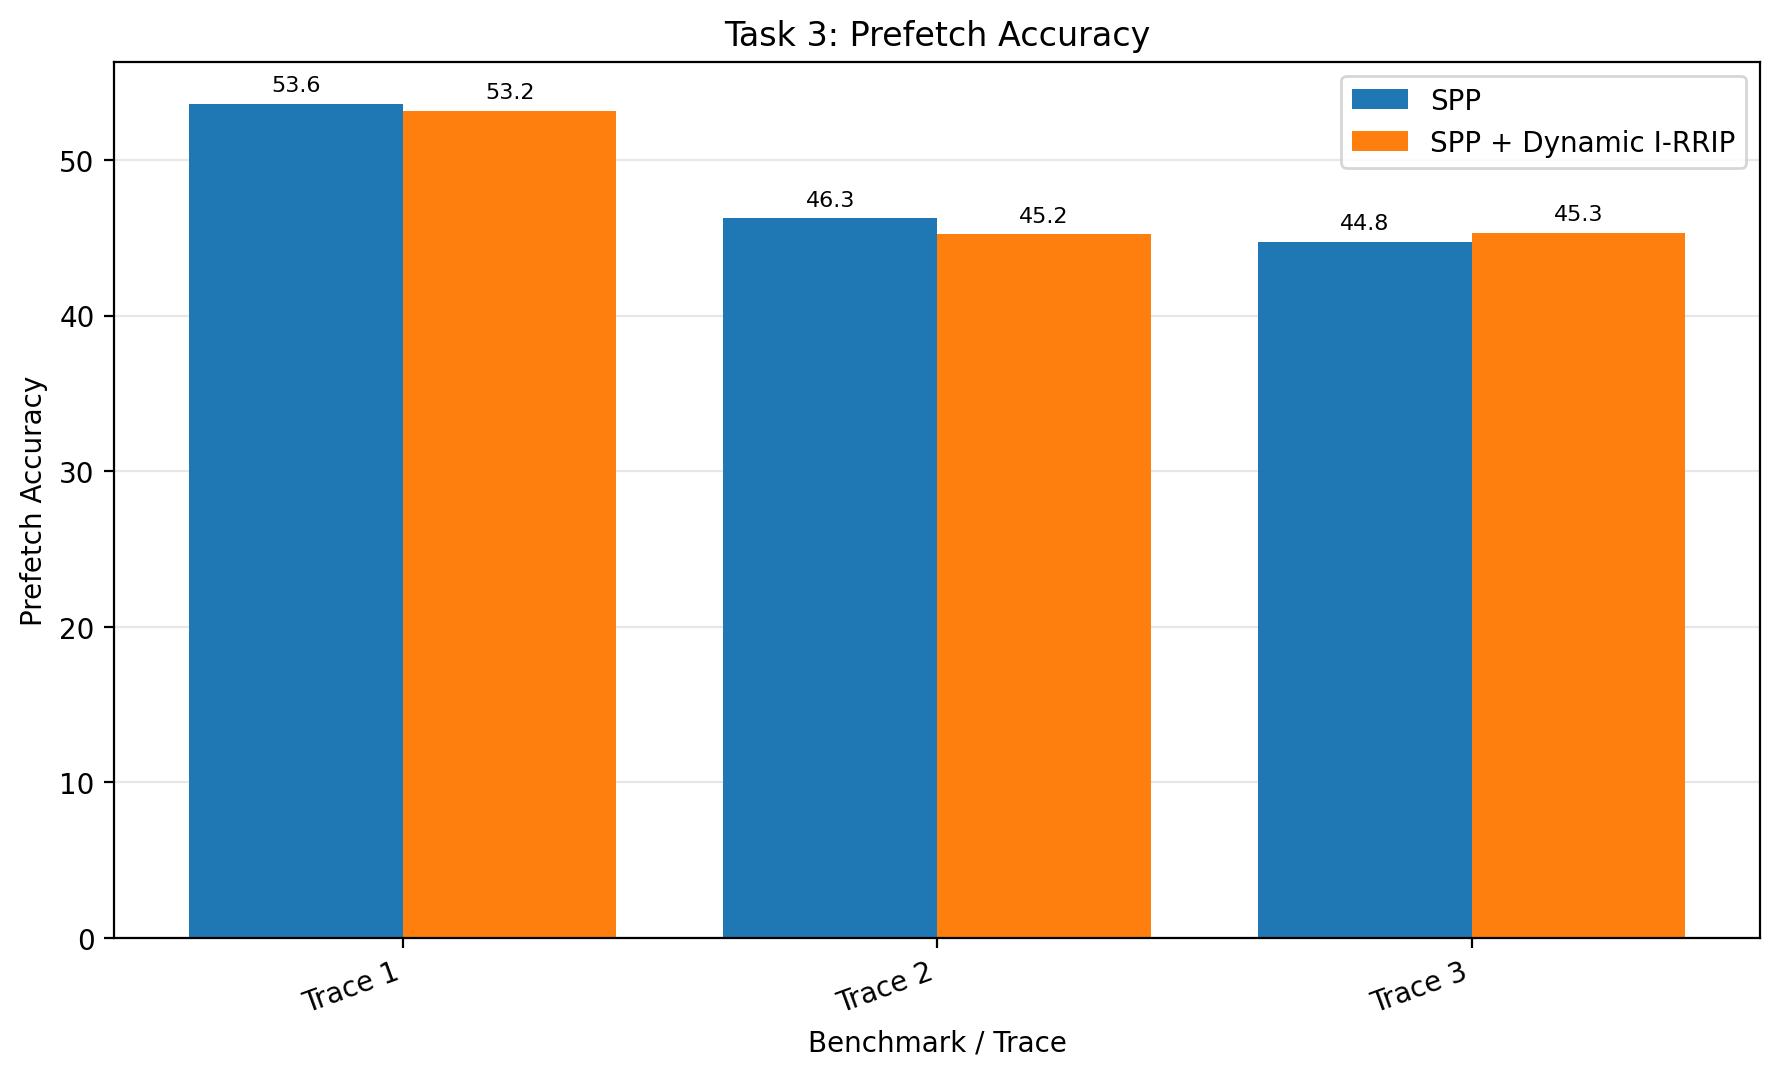
\includegraphics[width=\textwidth]{task3_accuracy.png}
        \caption{Prefetch Accuracy}
    \end{subfigure}
    \hfill
    \begin{subfigure}[b]{0.48\textwidth}
        \centering
        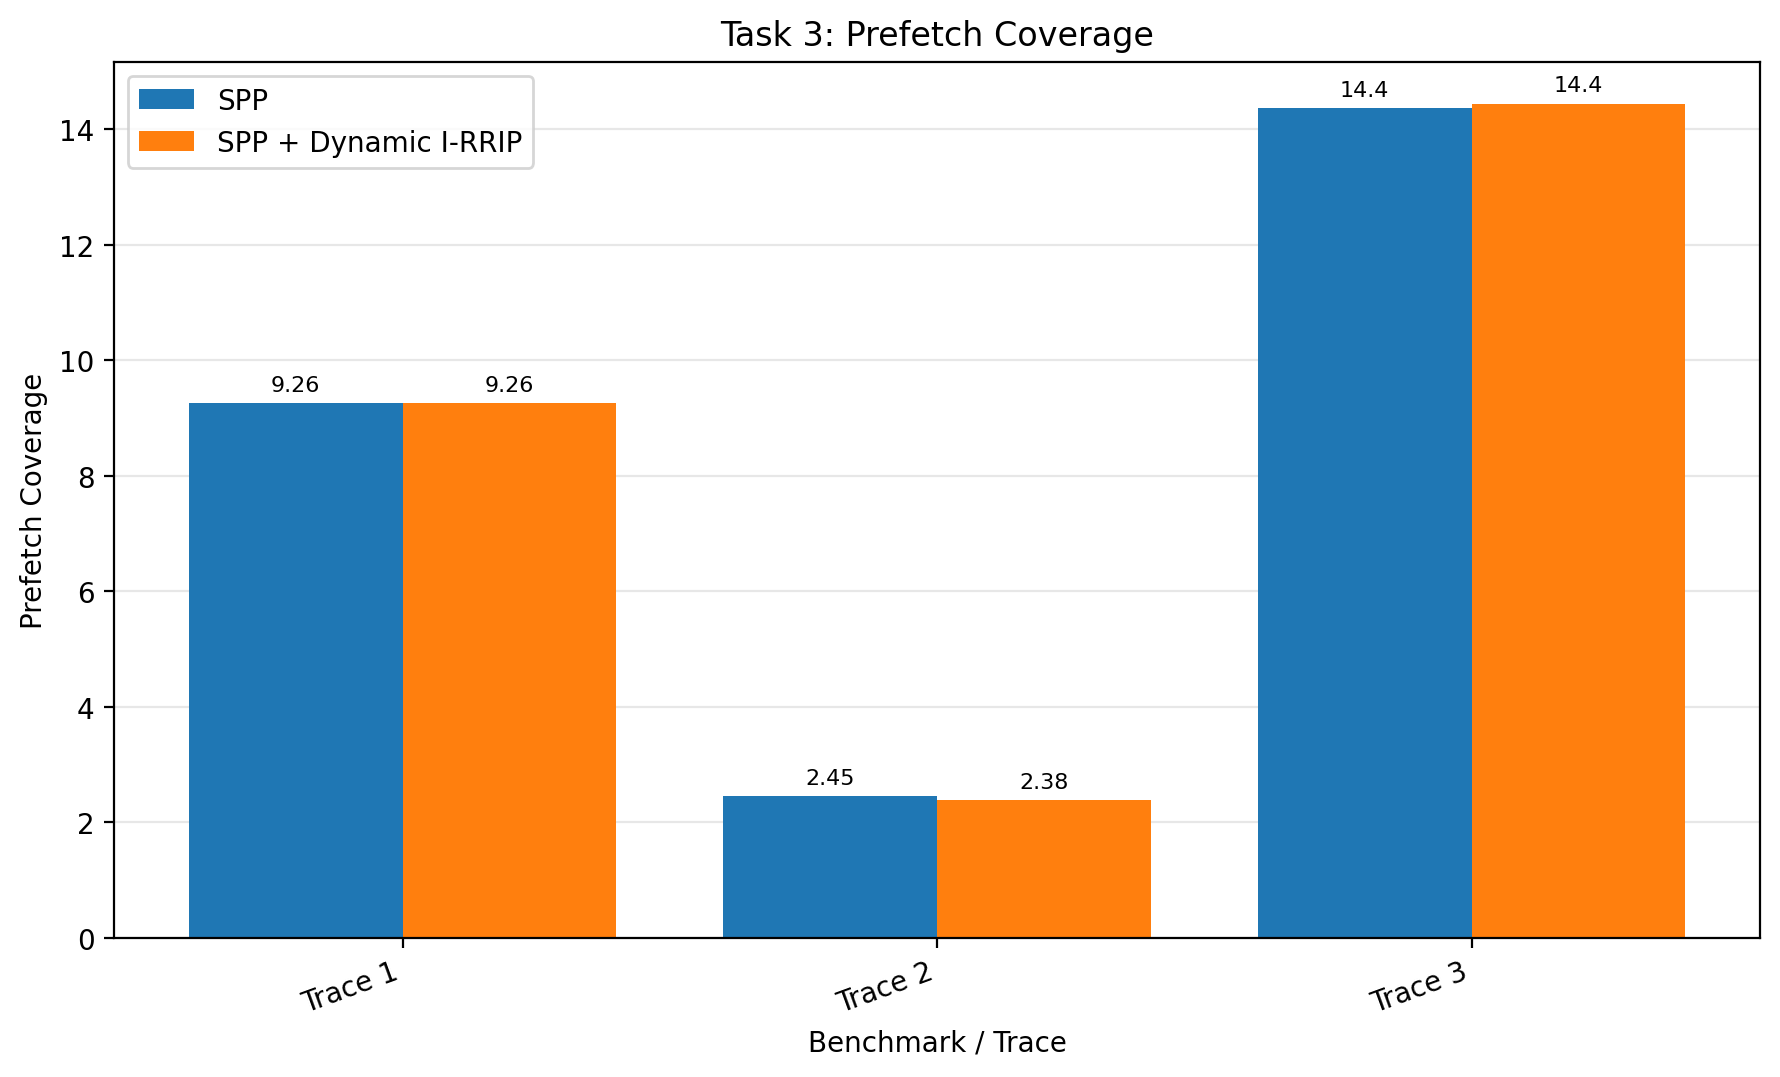
\includegraphics[width=\textwidth]{task3_coverage.png}
        \caption{Prefetch Coverage}
    \end{subfigure}
    \caption{Prefetch Accuracy and Coverage comparison between SPP and SPP + Dynamic I-RRIP.}
    \label{fig:task3-pref-acc-cov}
\end{figure}

\begin{figure}[H]
    \centering
    \begin{subfigure}[b]{0.48\textwidth}
        \centering
        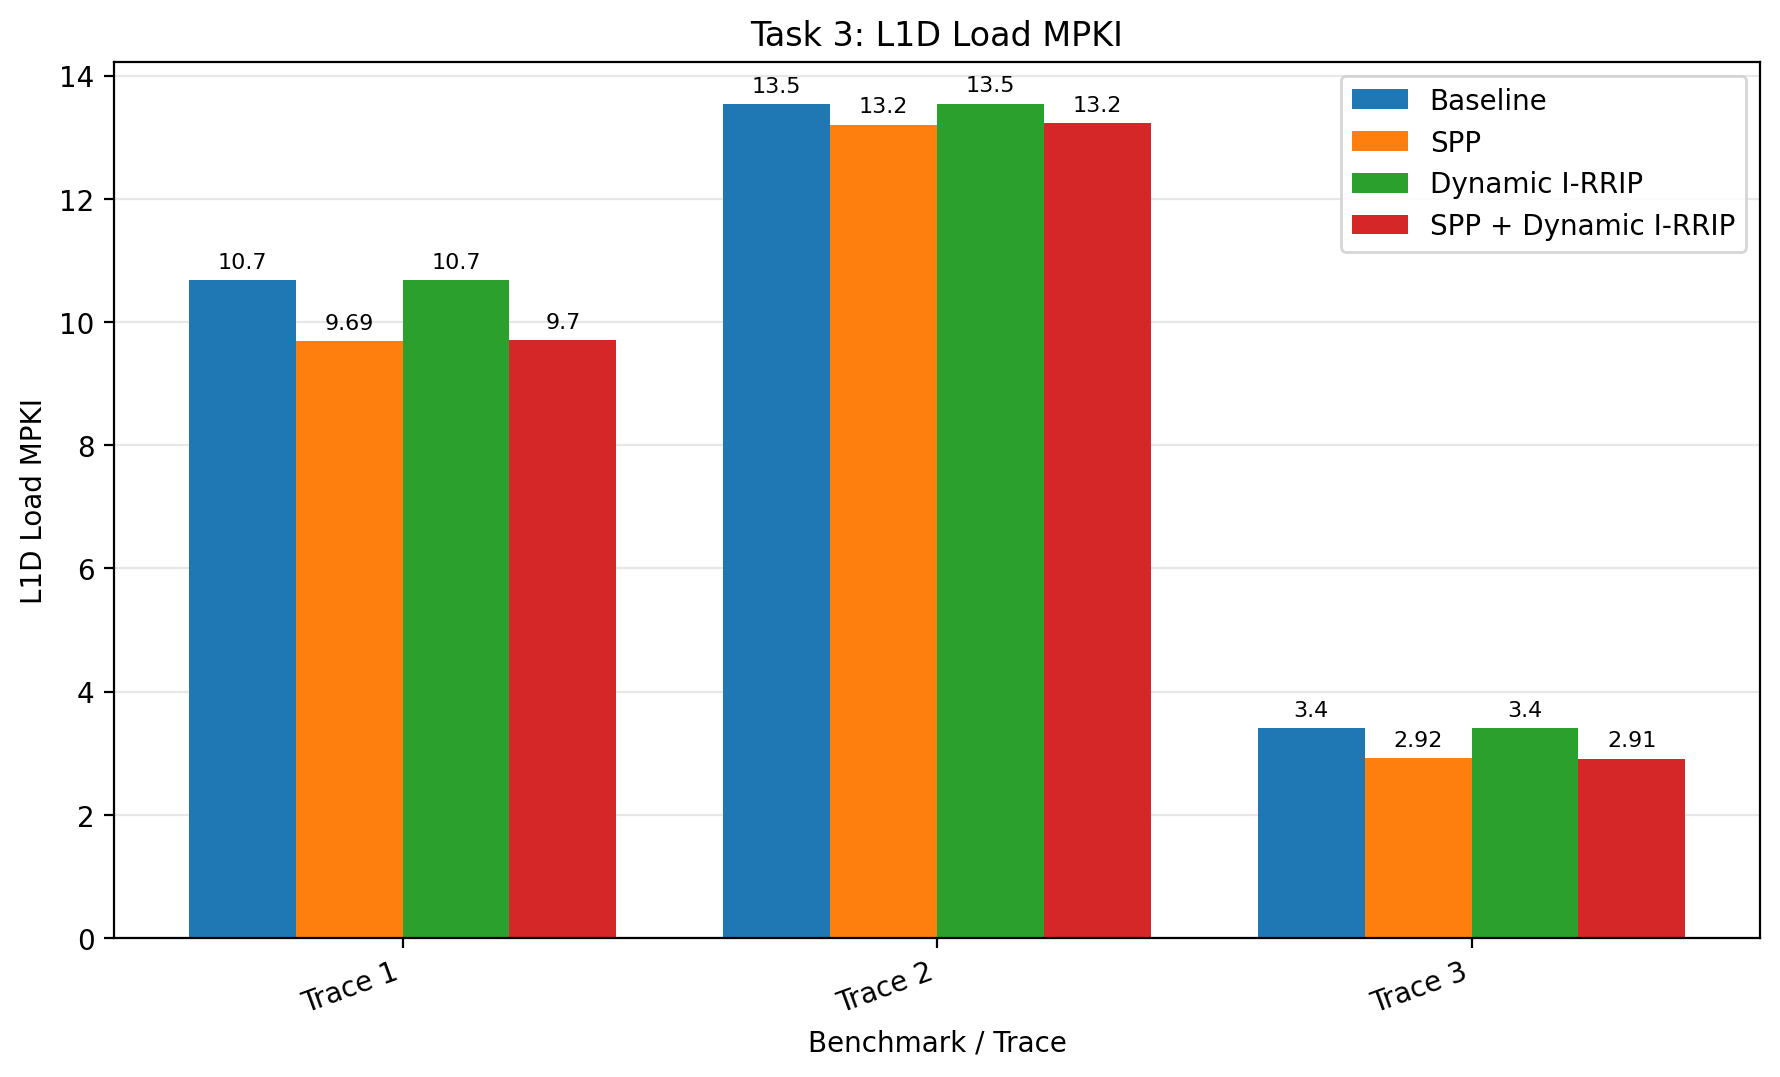
\includegraphics[width=\textwidth]{task3_l1d_load_mpki.png}
        \caption{L1D Load MPKI}
    \end{subfigure}
    \hfill
    \begin{subfigure}[b]{0.48\textwidth}
        \centering
        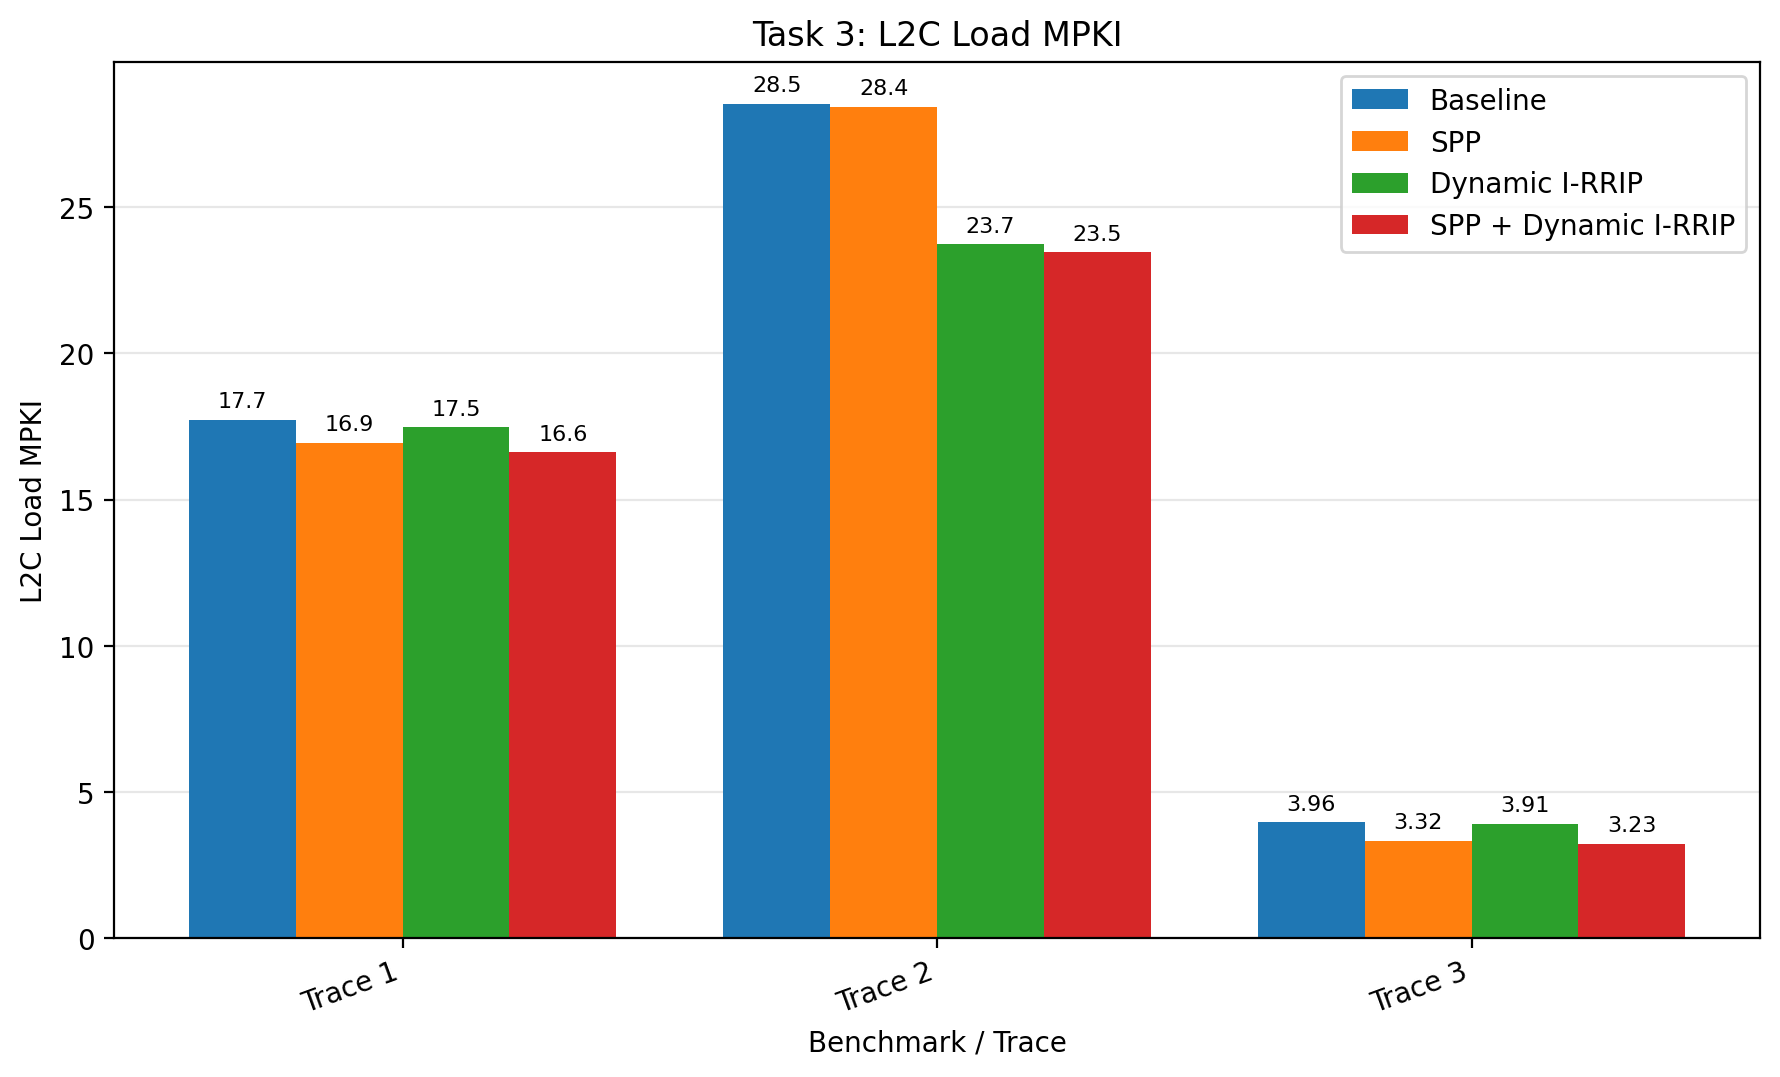
\includegraphics[width=\textwidth]{task3_l2c_load_mpki.png}
        \caption{L2C Total Load MPKI}
    \end{subfigure}
    \vskip\baselineskip
    \begin{subfigure}[b]{0.48\textwidth}
        \centering
        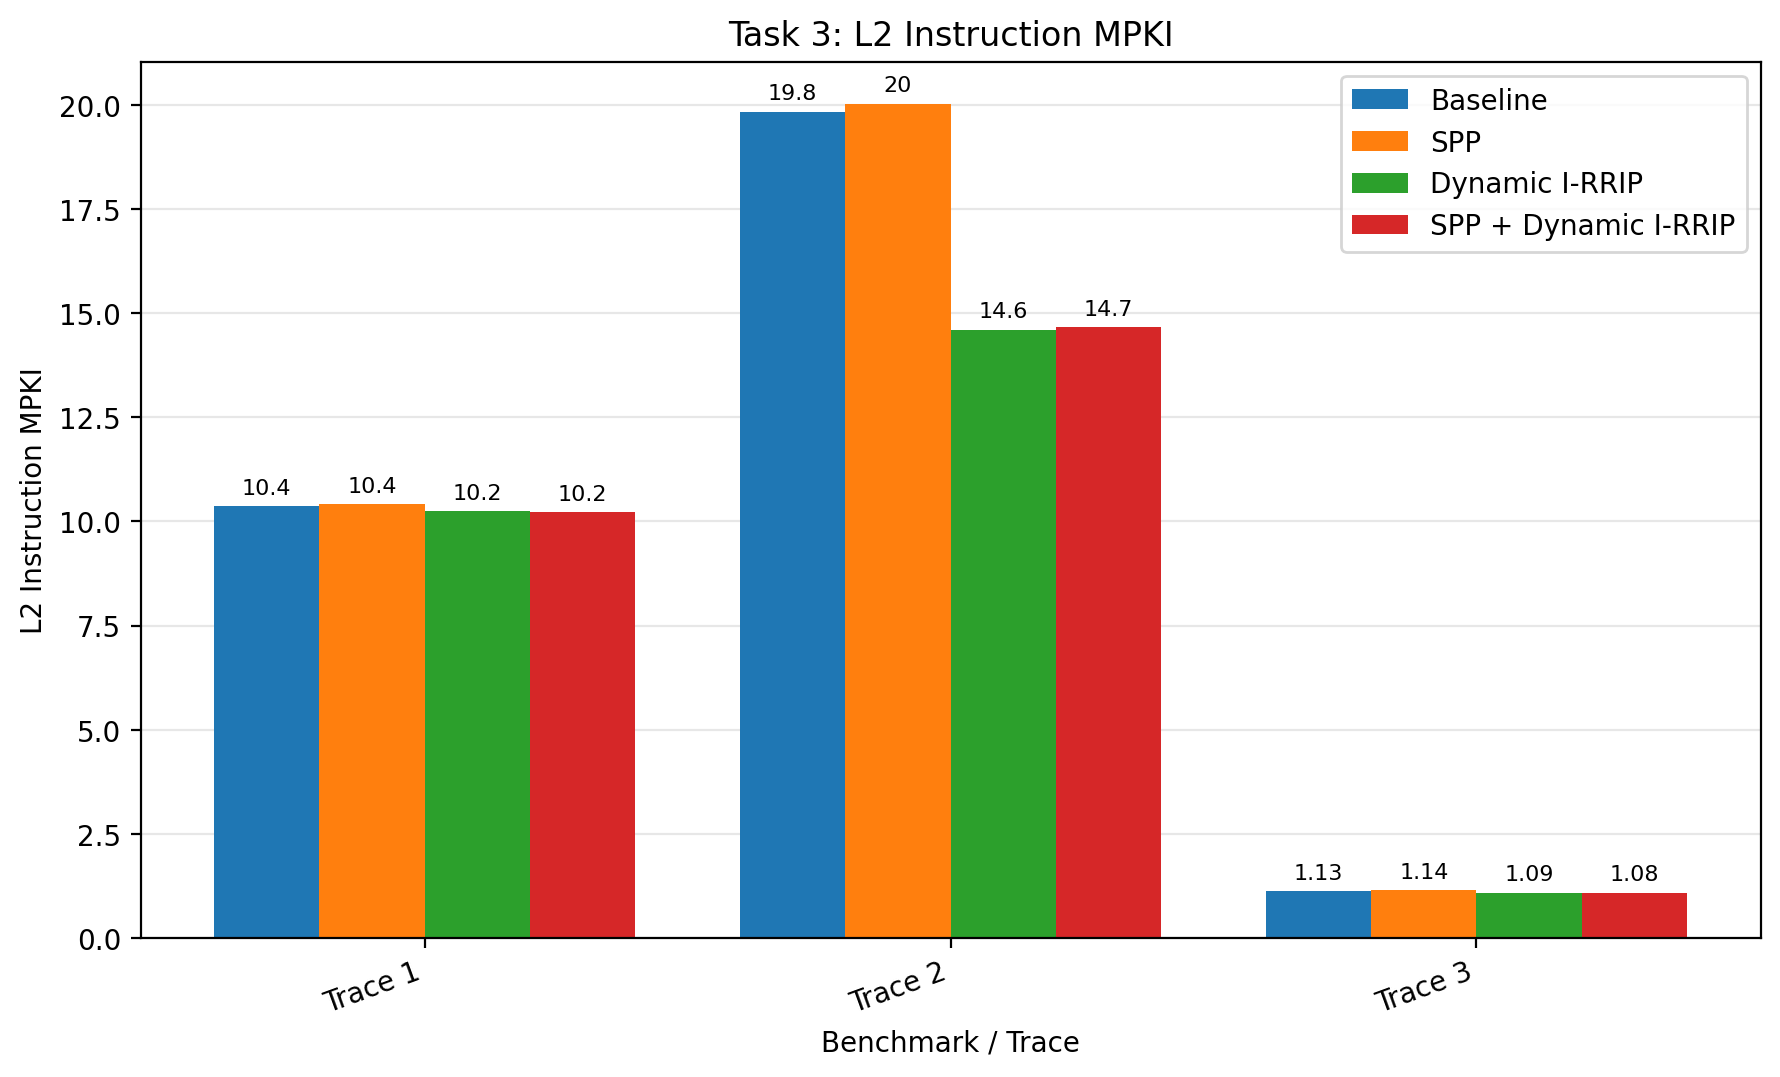
\includegraphics[width=\textwidth]{task3_l2i_load_mpki.png}
        \caption{L2 Instruction Load MPKI}
    \end{subfigure}
    \hfill
    \begin{subfigure}[b]{0.48\textwidth}
        \centering
        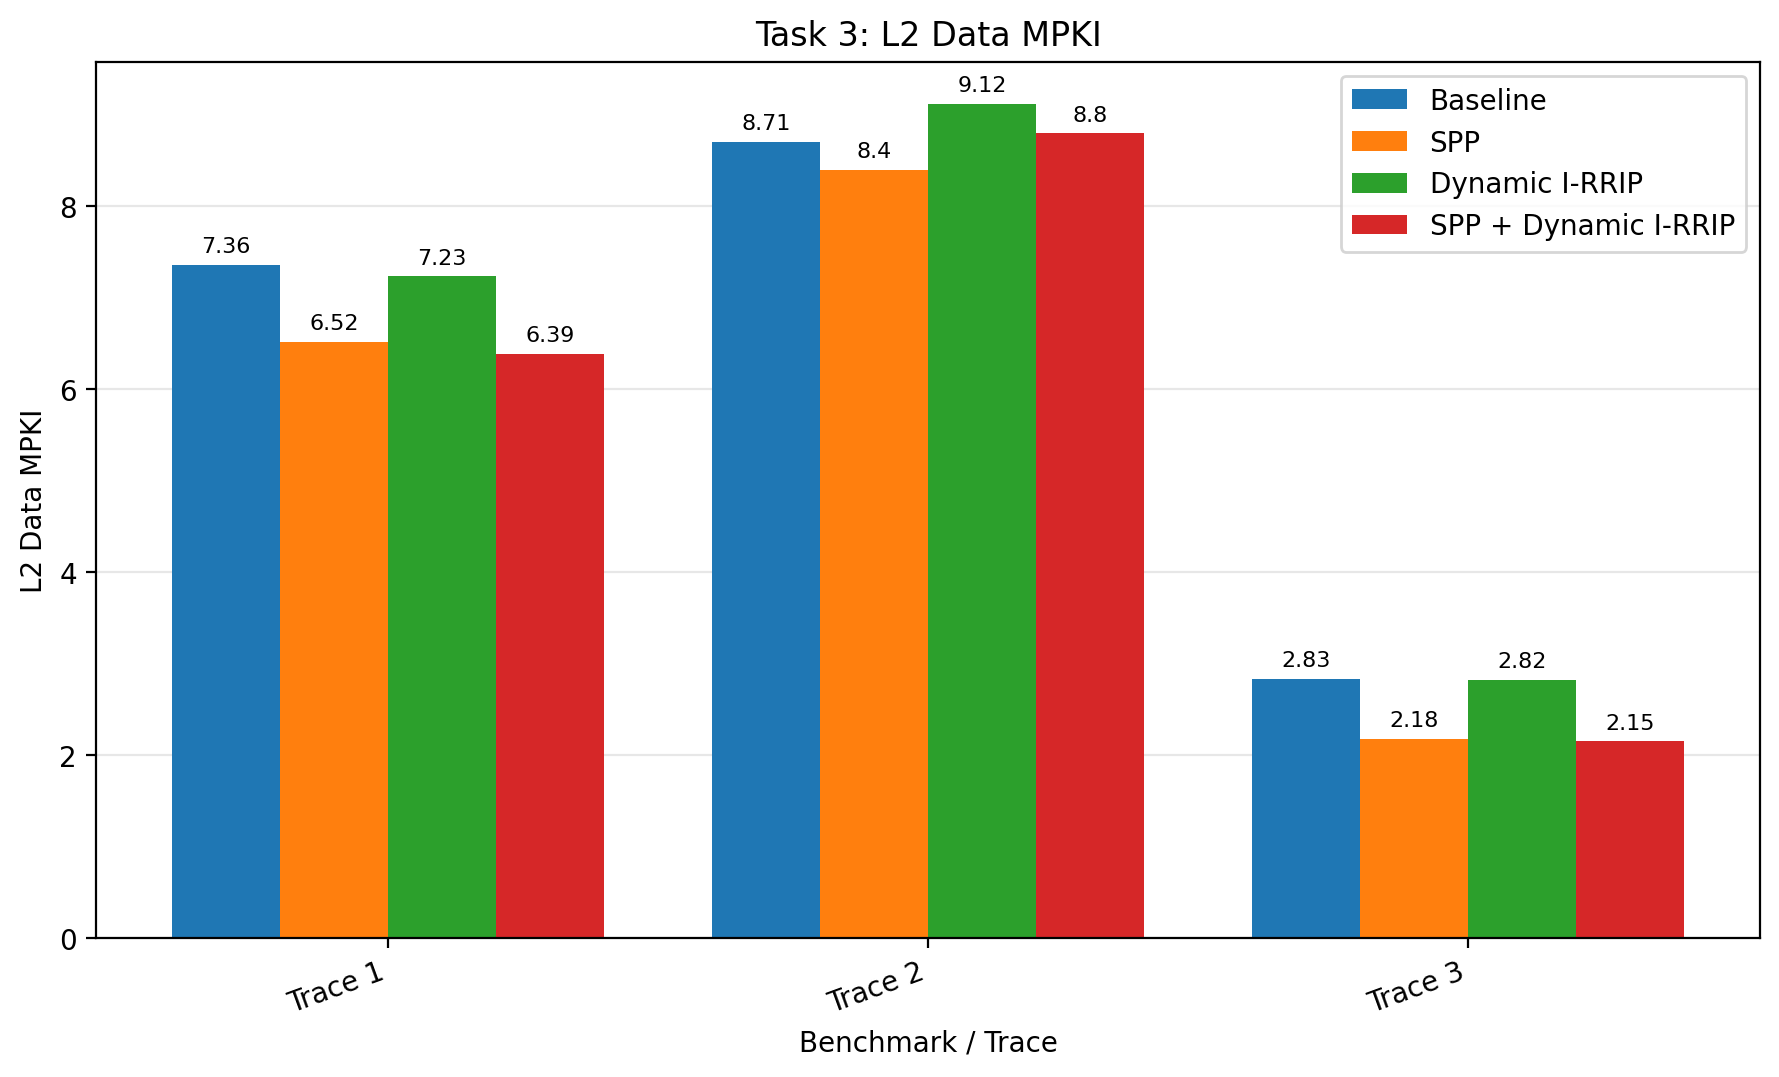
\includegraphics[width=\textwidth]{task3_l2d_load_mpki.png}
        \caption{L2 Data Load MPKI}
    \end{subfigure}
    \caption{Load MPKI breakdown across caches: L1D, L2C, L2 Instruction, and L2 Data.}
    \label{fig:task3-mpki-breakdown}
\end{figure}

\subsubsection{Rationale Behind Prefetch-Aware Replacement Policy}
When an aggressive data prefetcher like the Stride Pattern Prefetcher (SPP) operates at the L1D level alongside an instruction-conscious replacement policy at the L2 cache, naive cache replacement creates acute inter-stream interference:
\begin{itemize}
    \item \textbf{Preventing Instruction Eviction by Speculative Prefetches:} Prefetched data blocks brought into the cache hierarchy are speculative. If prefetch requests are inserted with high retention priority ($RRPV = 0$ or $1$), speculative prefetch streams can flood L2 sets and prematurely evict critical instruction lines. Because CPU execution strictly stalls on instruction cache misses, evicting instruction lines destroys the performance benefits achieved by prefetching.
    \item \textbf{Differentiated Insertion Policy ($RRPV = 2$):} In the prefetch-aware Dynamic I-RRIP policy, incoming cache blocks are inspected for their packet type. Demand instruction lines are prioritized with $RRPV = 1$, regular demand data lines are inserted with $RRPV = 2$, and prefetch lines (`type == PREFETCH`) are inserted with $RRPV = 2$ (distant re-reference prediction). This guarantees that speculative prefetch lines are placed at a distance from the MRU position and must prove their usefulness before displacing active instruction or demand data working sets.
    \item \textbf{Hit Promotion on Useful Demand Accesses ($RRPV = 0$):} When a prefetch block successfully experiences a demand hit (becoming a useful prefetch), it transitions to regular active data status and is promoted to $RRPV = 0$. This ensures that prefetches that successfully capture access patterns receive maximum retention priority.
    \item \textbf{Victim Selection Prioritization:} During eviction, lines with $RRPV = 3$ are chosen such that unreferenced prefetch lines are evicted before instruction lines or active demand data lines. This acts as an organic filtering mechanism that purges inaccurate or untimely prefetches without cache pollution.
    \item \textbf{Demonstrated Synergy and Performance Gains:} As evidenced by the results in Table~\ref{tab:task3-performance}, incorporating prefetch awareness enables the combined system to outperform both standalone SPP and standalone Dynamic I-RRIP across all benchmarks:
    \begin{itemize}
        \item On \textbf{Trace 1}, IPC increases to \textbf{0.2343} (+0.92\% speedup over baseline), surpassing both standalone SPP (0.2338) and standalone Dynamic I-RRIP (0.2324).
        \item On \textbf{Trace 2}, where instruction misses dominate, Dynamic I-RRIP slashes L2 Instruction MPKI from 19.84 to 14.67, while SPP simultaneously cuts L1D MPKI from 13.54 to 13.22. Working in concert with prefetch awareness, the combined policy reaches an IPC of \textbf{0.2564} (+2.55\% speedup), outperforming both standalone policies.
        \item On \textbf{Trace 3}, the combined system achieves the highest overall IPC of \textbf{0.3884} (+1.72\% speedup) with a minimal L1D MPKI of 2.91 and L2C MPKI of 3.23.
    \end{itemize}
\end{itemize}

 
\noindent\rule{\linewidth}{0.4pt}
\end{document}